%!TEX root = ../main.tex



\section{Εισαγωγή}

\lettrine[findent=2pt]{\fbox{\textbf{Σ}}}{ε} αυτό το κεφάλαιο θα παρουσιαστούν τα πειράματα που έγιναν έτσι ώστε να υπάρχει εφαρμογή της θεωρίας στην πράξη όσων έχουν αναφερθεί στα προηγούμενα κεφάλαια. Με αυτόν τον τρόπο μελετάται και κατά πόσο ο ελεγκτής που σχεδιάστηκε είναι ικανός να ελέγξει ικανοποιητικά διάφορα συστήματα ελέγχου. Σε κάθε ενότητα θα παρουσιάζεται ένα από τα διαθέσιμα συστήματα, το μαθηματικό μοντέλο του και τα αποτελέσματα του ελέγχου που παρέχει ο αυτο-ρυθμιζόμενος PID ελεγκτής. Τέλος, η κάθε ενότητα κλείνει με το σχολιασμό των πειραματικών αποτελεσμάτων.

\section{Σύστημα Mass-Spring-Damper}

\subsection{Μαθηματικό Μοντέλο}

Το πρώτο σύστημα που θα αναλυθεί είναι το σύστημα Μάζα-Ελατήριο-Αποσβεστήρας (Σχήμα \ref{fig:mass_spring_damper}) που αποτελεί ένα από τα πιο κλασικά συστήματα ελέγχου καθώς οι δυναμικές σχέσεις που το διέπουν δεν είναι περίπλοκες και είναι εύκολη η κατανόηση τους.

\begin{figure}[h]
  \centering
  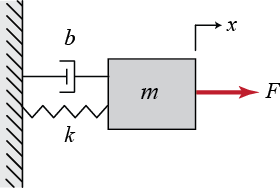
\includegraphics[width=\textwidth,height=5cm,keepaspectratio]{mass_spring_damper}
  \caption{Μοντέλο συστήματος Μάζας-Ελατηρίου-Αποσβεστήρα}
  \label{fig:mass_spring_damper}
\end{figure}

\noindent
H διαφορική εξίσωση που χαρακτηρίζει το σύστημα αυτό είναι
\begin{equation}
m\ddot{x} + b\dot{x} + kx = F
\label{eq:mass_springer_damper_ode}
\end{equation}
όπου $m$ είναι η μάζα, $x$ είναι η μετατόπιση της μάζας από το σημείο ισορροπίας, $b$ είναι η απόσβεση που παρέχει ο αποσβεστήρας, $k$ είναι η σταθερά του ελατηρίου και $F$ είναι η δύναμη που ασκείται στο σύστημα. Παίρνοντας το μετασχηματισμό Laplace της παραπάνω εξίσωσης έχουμε
\begin{equation}
ms^2X(s) + bsX(s) + kX(s) = F(s)
\label{eq:mass_springer_damper_laplace}
\end{equation}
Συνεπώς η συνάρτηση μεταφοράς (\emph{Transfer Function}) μεταξύ της εισόδου, που είναι η δύναμη $F(s)$, και της εξόδου, που είναι η μετατόπιση της μάζας $X(s)$, είναι
\begin{equation}
\frac{X(s)}{F(s)} = \frac{1}{ms^2 + bs + k}
\end{equation}

\subsection{Πείραμα}

Έστω ότι $\displaystyle m = 1\ kg$, $\displaystyle b = 10\ \frac{Ns}{m}$, $\displaystyle k = 20\ \frac{N}{m}$, $\displaystyle F = 1\ N$. Αντικαθιστώντας αυτές τις τιμές στην εξίσωση \ref{eq:mass_springer_damper_laplace} έχουμε
\begin{equation}
\frac{X(s)}{F(s)} = \frac{1}{s^2 + 10s + 20}
\end{equation}

\subsubsection{Απόκριση Χωρίς Έλεγχο}

Στο Σχήμα \ref{fig:mass_springer_damper_no_control} φαίνεται η βηματική απόκριση του συστήματος όταν δεν υπάρχει έλεγχος. Καθίσταται εμφανές ότι από μόνο του το σύστημα έχει μη ικανοποιητική απόκριση καθώς η τελική τιμή της εξόδου του είναι $y(t) = 0,047619$ και έχει ποσοστό σφάλματος \textit{offset error}$= 95.238 \%$. Συνεπώς κρίνεται απαραίτητη η χρήση ελεγκτή. Τα κέρδη του θα υπολογιστούν χρησιμοποιώντας τη μέθοδο αυτο-ρύθμισης που έχει περιγραφεί.

\begin{figure}[h]
  \centering
  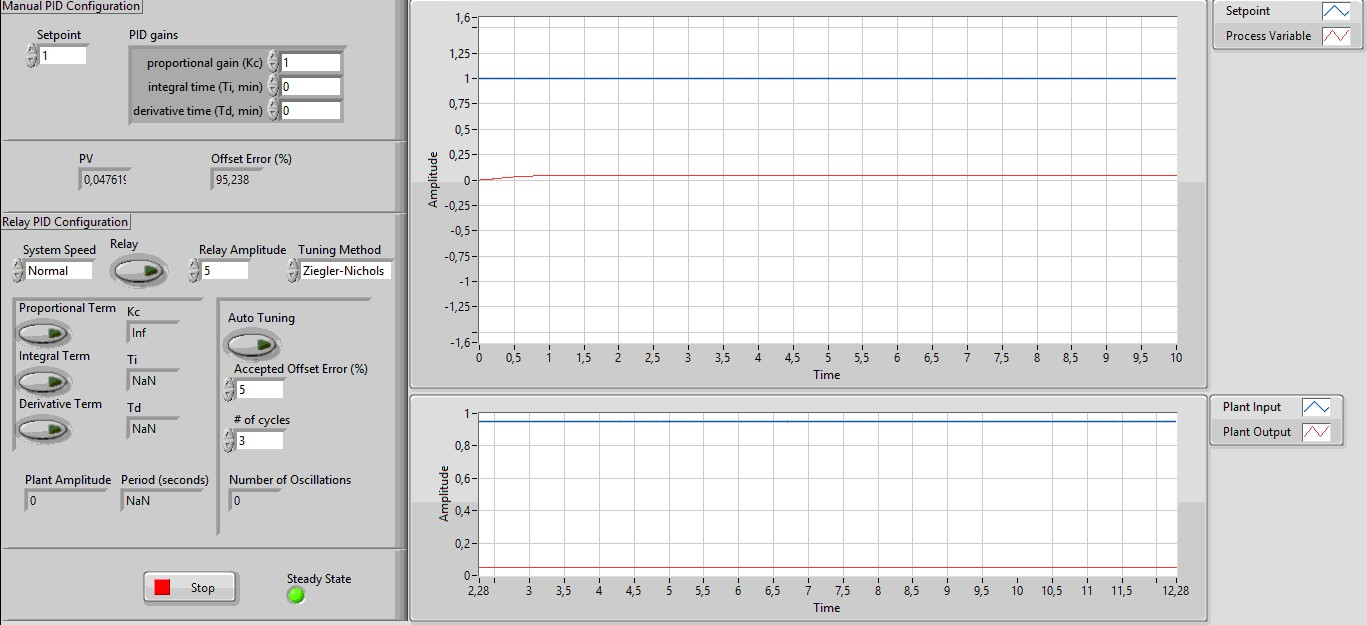
\includegraphics[width=\textwidth,height=5cm,keepaspectratio]{mass_springer_damper_no_control}
  \caption{Βηματική απόκριση του συστήματος Μάζα-Ελατήριο-Αποσβεστήρας χωρίς έλεγχο}
  \label{fig:mass_springer_damper_no_control}
\end{figure}

\subsubsection{Αναλογικός Έλεγχος}

Στο Σχήμα \ref{fig:mass_springer_damper_proportional_control} φαίνεται η βηματική απόκριση του συστήματος όταν σε αυτό εφαρμόζεται αναλογικός έλεγχος. Το κέρδος $K_c$ του αναλογικού όρου υπολογίστηκε αυτόματα, χρησιμοποιώντας τους τύπους από τη μέθοδο Ziegler-Nichols. Βλέπουμε ότι με τη χρήση του αναλογικού ελέγχου το σφάλμα βελτιώθηκε στο βαθμό η τελική τιμή του συστήματος να έχει πλέον μόνο $3,624\%$ απόκλιση από την επιθυμητή τιμή, αλλά, όπως είχε αναφερθεί και στην ενότητα \ref{subsec:proportional_control}, δεν μπορεί να το μηδενίσει. Επίσης, ο έλεγχος εισήγαγε ταλαντώσεις και υπέρβαση κατά ένα ποσοστό περίπου $50\%$. Αυτό, ανάλογα με τις απαιτήσεις ελέγχου, μπορεί να μην είναι αποδεκτό.

Στο ίδιο σχήμα φαίνεται η αριθμητική τιμή του πλάτους και της περιόδου των ταλαντώσεων που υπολόγισε ο αλγόριθμος. Το Σχήμα \ref{fig:mass_springer_damper_oscillations} αποτελεί μεγέθυνση του \ref{fig:mass_springer_damper_proportional_control} και αποδεικνύει ότι ο αλγόριθμος είναι πολύ ακριβής στην εύρεση των χαρακτηριστικών των ταλαντώσεων. 

\begin{figure}[h]
  \centering
  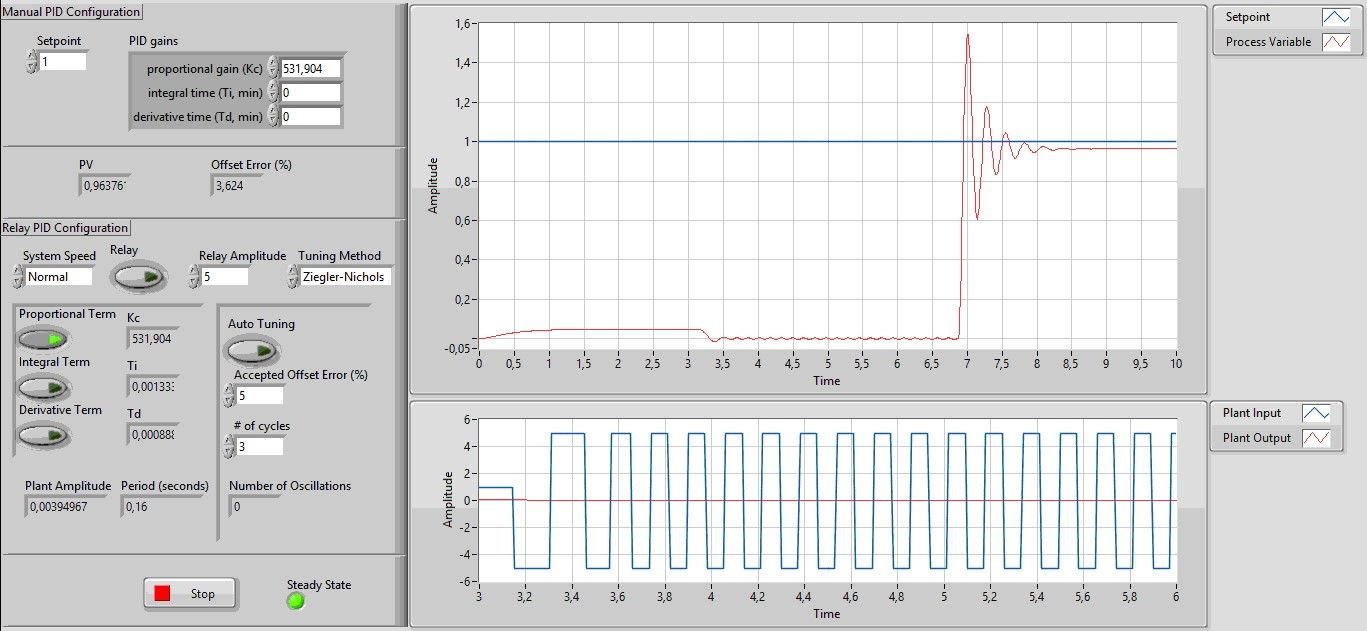
\includegraphics[width=\textwidth,height=5cm,keepaspectratio]{mass_springer_damper_proportional_control}
  \caption{Βηματική απόκριση του συστήματος Μάζα-Ελατήριο-Αποσβεστήρας με εφαρμογή αναλογικού ελέγχου}
  \label{fig:mass_springer_damper_proportional_control}
\end{figure}

\begin{figure}[h]
  \centering
  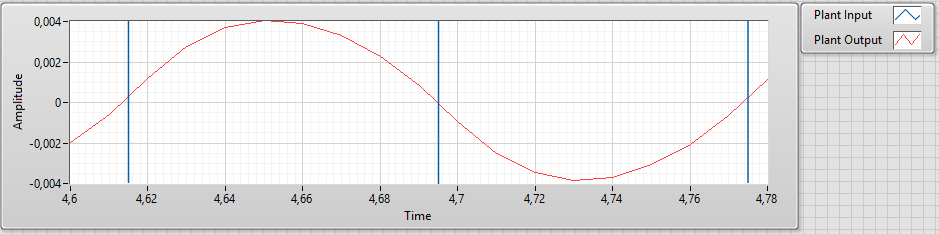
\includegraphics[width=\textwidth]{mass_springer_damper_oscillations}
  \caption{Μεγέθυνση των ταλαντώσεων του συστήματος κατά τη διάρκεια του πειράματος relay}
  \label{fig:mass_springer_damper_oscillations}
\end{figure}

\subsubsection{Αναλογικός-Ολοκληρωτικός Έλεγχος}

Το πείραμα επαναλαμβάνεται αλλά αυτή τη φορά χρησιμοποιείται και ο ολοκληρωτικός όρος προκειμένου να εξαλειφθεί το σφάλμα μόνιμης κατάστασης. Όπως φαίνεται από το Σχήμα \ref{fig:mass_springer_damper_integral_control}, η προσθήκη του ολοκληρωτικού όρου, όχι μόνο δεν μηδενίζει το σφάλμα μόνιμης κατάστασης αλλά χειροτερεύει την απόκριση του συστήματος σε σημείο να το οδηγεί να εκτελεί ταλαντώσεις γύρω από το επιθυμητό σημείο. Αυτό χωρίς αμφιβολία, είναι μία μη αποδεκτή κατάσταση.

\begin{figure}[h]
  \centering
  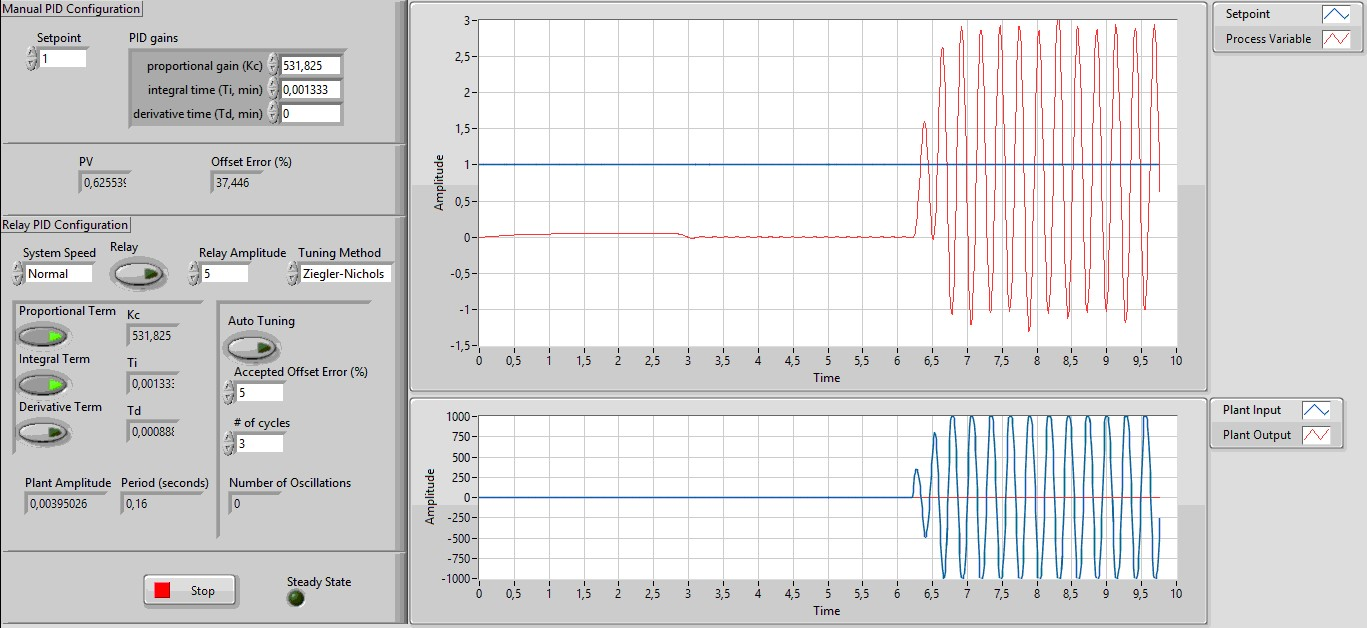
\includegraphics[width=\textwidth,height=5cm,keepaspectratio]{mass_springer_damper_integral_control}
  \caption{Βηματική απόκριση του συστήματος Μάζα-Ελατήριο-Αποσβεστήρας με εφαρμογή αναλογικού-ολοκληρωτικού ελέγχου}
  \label{fig:mass_springer_damper_integral_control}
\end{figure}

\subsubsection{Αναλογικός-Ολοκληρωτικός-Διαφορικός Έλεγχος}

Προκειμένου να βελτιωθεί η ευστάθεια του συστήματος εισάγεται και ο διαφορικός όρος. Ενώ ο ολοκληρωτικός όρος εισάγει έναν πόλο στο σύστημα, ο διαφορικός όρος εισάγει ένα μηδενικό βελτιώνοντας έτσι την ευστάθεια. Όπως φαίνεται στο Σχήμα \ref{fig:mass_springer_damper_derivative_control} η απόκριση βελτιώθηκε αισθητά. Ο έλεγχος που παρέχουν και οι τρεις όροι, όχι μόνο μηδένισε το σφάλμα μόνιμης κατάστασης όπως ήταν αναμενόμενο λόγω του ολοκληρωτικού όρου, αλλά βελτίωσε και τη μεταβατική κατάσταση του συστήματος. Η υπέρβαση, που πριν είχε ποσοστό σχεδόν $50\%$ τώρα έχει ποσοστό περίπου $20\%$. Επίσης έχει χρόνο ανύψωσης λιγότερο από ένα δευτερόλεπτο. Πλέον η απόκριση του συστήματος κρίνεται ικανοποιητική.

\begin{figure}[h]
  \centering
  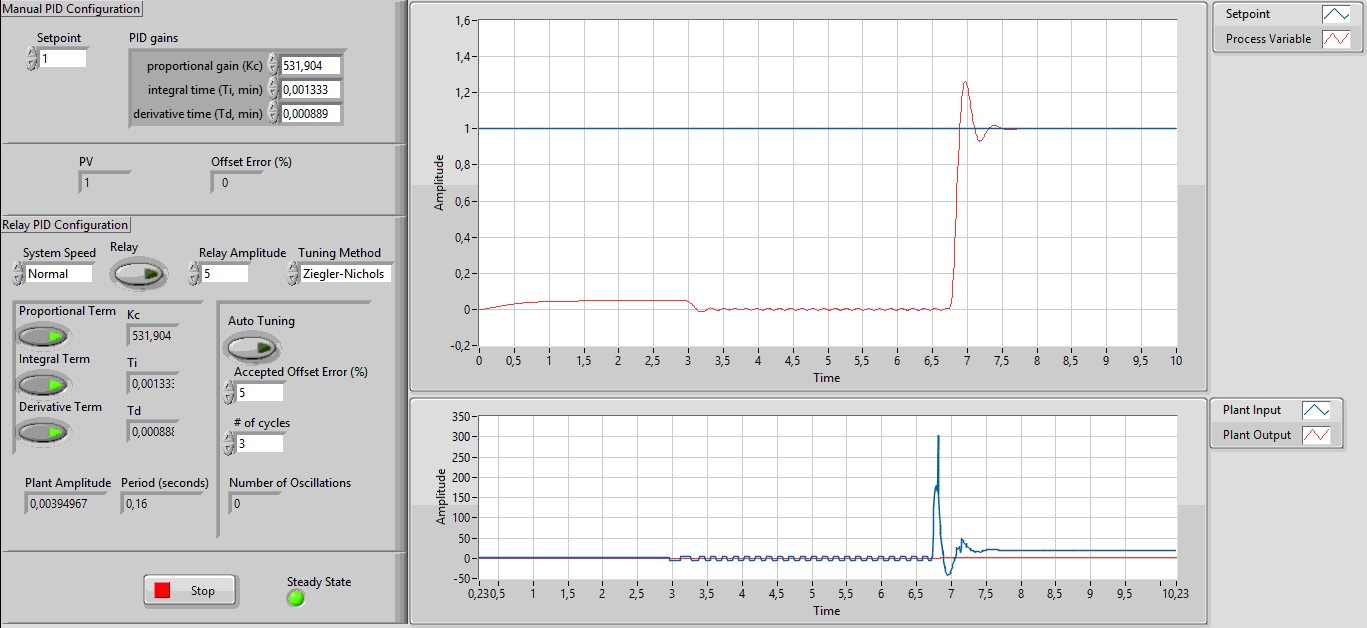
\includegraphics[width=\textwidth,height=5cm,keepaspectratio]{mass_springer_damper_derivative_control}
  \caption{Βηματική απόκριση του συστήματος Μάζα-Ελατήριο-Αποσβεστήρας με εφαρμογή αναλογικού-ολοκληρωτικού-διαφορικού ελέγχου}
  \label{fig:mass_springer_damper_derivative_control}
\end{figure}

Όπως έχει αναφερθεί κάθε διεργασία μπορεί να έχει διαφορετικές απαιτήσεις ελέγχου. Μπορεί για μία συγκεκριμένη εφαρμογή, η υπέρβαση που παρουσιάζει ο έλεγχος με αυτά τα κέρδη να μην είναι αποδεκτός. Έχει ενδιαφέρον λοιπόν να δούμε πώς ανταποκρίνεται το σύστημα σε διαφορετικές τιμές των κερδών. Ορίζοντας την επιθυμητή ταχύτητα του κλειστού συστήματος σε ``Slow" αντί για ``Normal" έχουμε την παρακάτω απόκριση. Από το διάγραμμα βλέπουμε ότι πλέον το σύστημα δεν παρουσιάζει υπέρβαση αλλά ως αντάλλαγμα αργεί αισθητά περισσότερο να φτάσει στην επιθυμητή τιμή.

\begin{figure}[h]
  \centering
  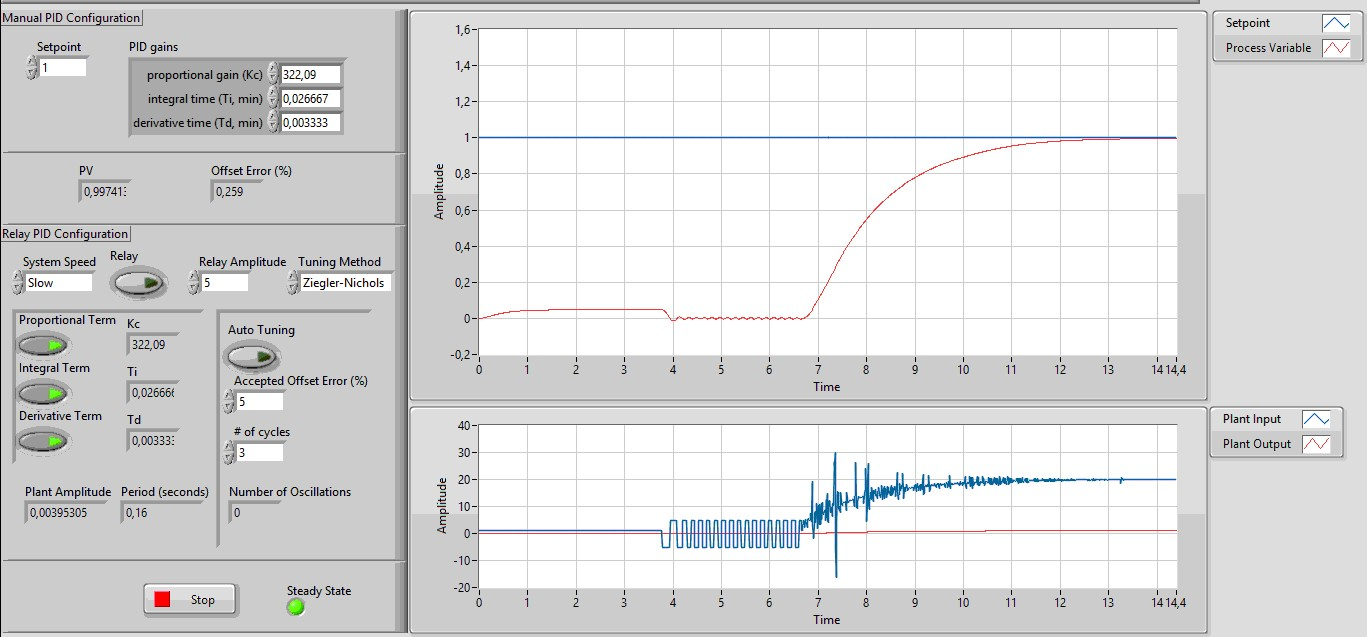
\includegraphics[width=\textwidth,height=5cm,keepaspectratio]{mass_springer_damper_ZN_slow}
  \caption{Βηματική απόκριση του συστήματος Μάζα-Ελατήριο-Αποσβεστήρας με εφαρμογή αναλογικού-ολοκληρωτικού-διαφορικού ελέγχου στη λειτουργία ``Slow"}
  \label{fig:mass_springer_damper_ZN_slow}
\end{figure}

Ακόμα, στο Σχήμα \ref{fig:mass_springer_damper_TL} φαίνεται η βηματική απόκριση του κλειστού συστήματος όταν τα κέρδη του ελεγκτή έχουν υπολογιστεί με τους τύπους Tyreus-Luyben. Η απόκριση μοιάζει σαν μια μίξη των δύο προηγούμενων αποκρίσεων. Η έξοδος του συστήματος δεν παρουσιάζει υπέρβαση, αλλά φτάνει και στην επιθυμητή τιμή μέσα σε περίπου ένα δευτερόλεπτο.

\begin{figure}[h]
  \centering
  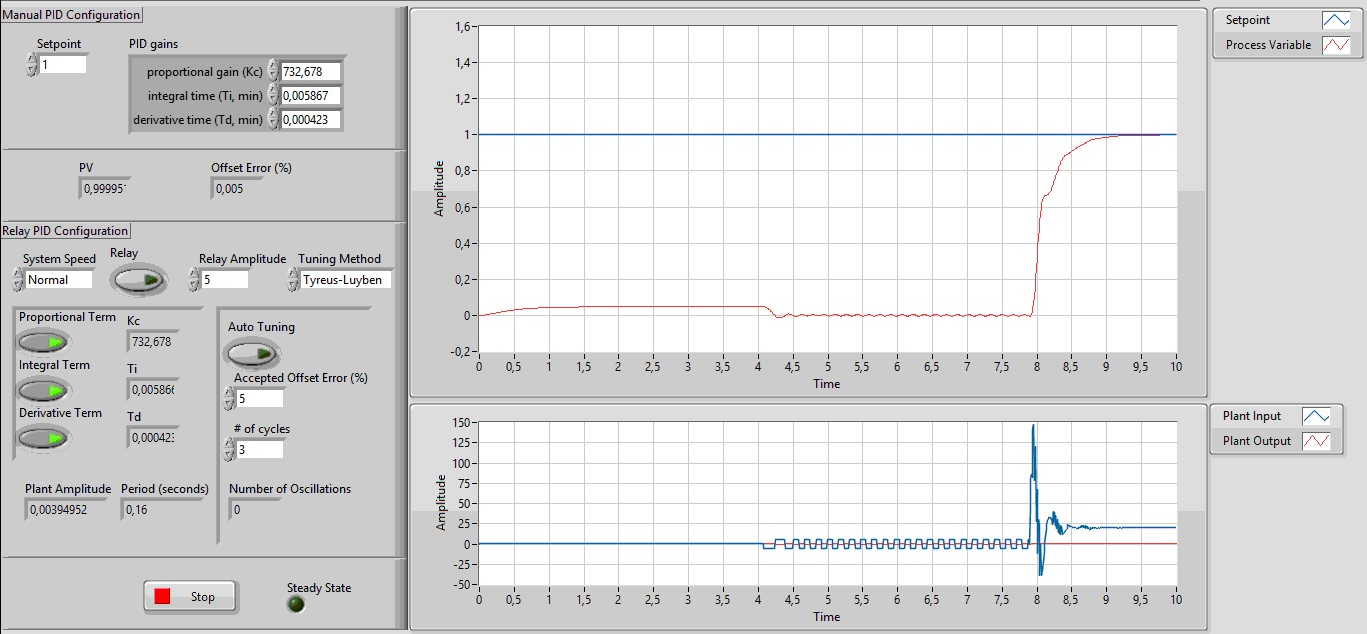
\includegraphics[width=\textwidth,height=5cm,keepaspectratio]{mass_springer_damper_TL}
  \caption{Βηματική απόκριση του συστήματος Μάζα-Ελατήριο-Αποσβεστήρας με εφαρμογή αναλογικού-ολοκληρωτικού-διαφορικού ελέγχου του οποίου τα κέρδη έχουν υπολογιστεί με τους τύπους Tyreus-Luyben}
  \label{fig:mass_springer_damper_TL}
\end{figure}



\subsubsection{Αντιμετώπιση Διαταραχών}
Στο Σχήμα \ref{fig:mass_spring_damper_disturbances} φαίνεται πώς το σύστημα αντιδράει στην ύπαρξη διαταραχών. Περίπου στο δέκατο τρίτο δευτερόλεπτο, γίνεται μια γρήγορη μεταβολή του setpoint η οποία ισοδυναμεί με μία σχεδόν στιγμιαία διαταραχή. Από το διάγραμμα της απόκρισης φαίνεται ότι το σύστημα έχει επανέλθει στην ηρεμία και έχει μηδενικό σφάλμα μόνιμης κατάστασης. 

\begin{figure}[h]
  \centering
  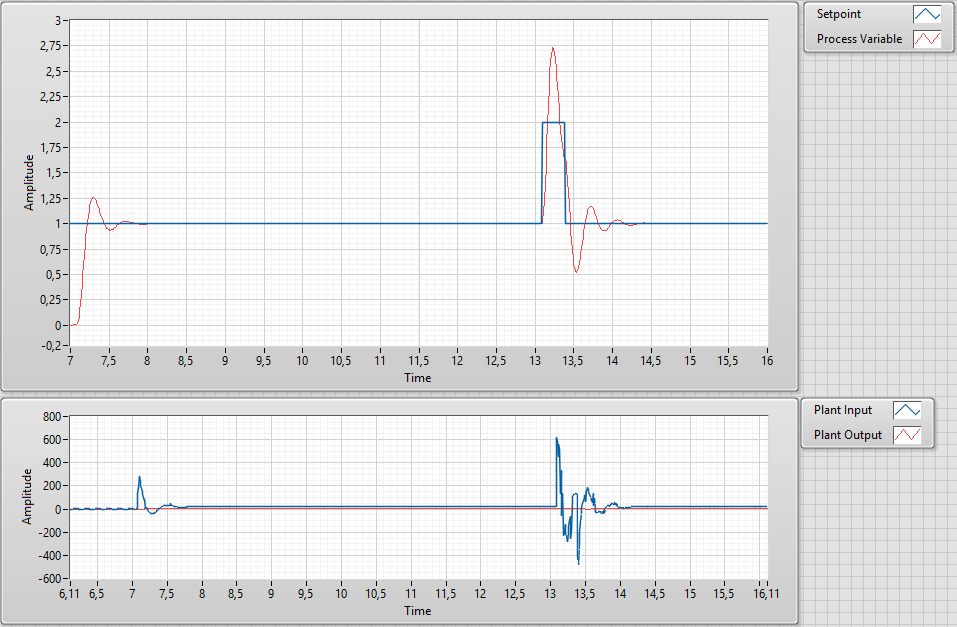
\includegraphics[width=\textwidth,height=5cm,keepaspectratio]{mass_spring_damper_disturbances}
  \caption{Αντιμετώπιση διαταραχών του αυτο-ρυθμιζόμενου PID ελεγκτή του οποίου τα κέρδη έχουν υπολογιστεί με τους τύπους Ziegler-Nichols}
  \label{fig:mass_spring_damper_disturbances}
\end{figure}

Όπως και πριν, έχει ενδιαφέρον να δούμε πώς διαχειρίζεται τις διαταραχές το σύστημα όταν τα κέρδη του ελεγκτή έχουν υπολογιστεί χρησιμοποιώντας διαφορετικούς τύπους. Έτσι, στο Σχήμα \ref{fig:mass_spring_damper_disturbances_slow} φαίνεται η προσπάθεια του ελεγκτή να ελέγξει το σύστημα σε διαταραχή, όταν τα κέρδη έχουν υπολογιστεί με τη μέθοδο Ziegler-Nichols και οι τύποι έχουν προσαρμοστεί για να δίνουν μια πιο αργή απόκριση.

\begin{figure}[h]
  \centering
  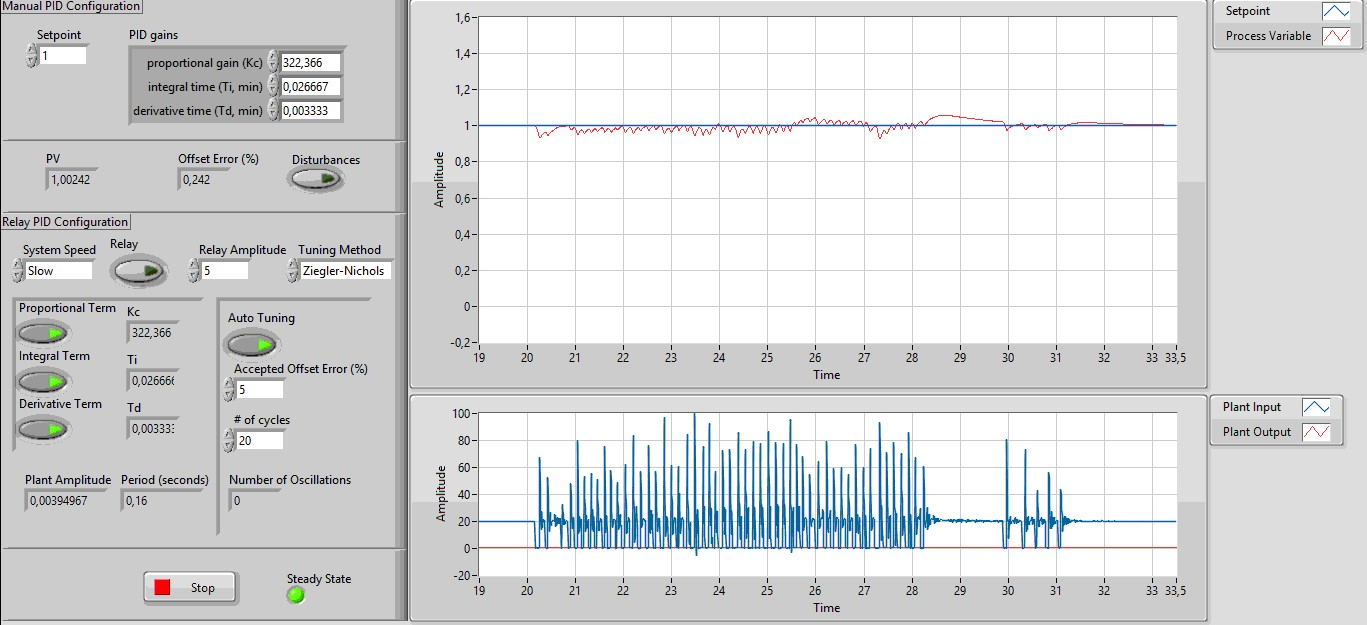
\includegraphics[width=\textwidth,height=5cm,keepaspectratio]{mass_spring_damper_disturbances_slow}
  \caption{Αντιμετώπιση διαταραχών του αυτο-ρυθμιζόμενου PID ελεγκτή του οποίου τα κέρδη έχουν υπολογιστεί με τους τύπους Ziegler-Nichols στη λειτουργία ``Slow"}
  \label{fig:mass_spring_damper_disturbances_slow}
\end{figure}

Τέλος, στο Σχήμα \ref{fig:mass_spring_damper_disturbances_TL} φαίνεται η αντιμετώπιση των διαταραχών όταν τα κέρδη έχουν υπολογιστεί με τους τύπους Tyreus-Luyben. Το σύστημα σταθεροποιείται πριν περάσει περισσότερο από ένα δευτερόλεπτο αλλά παρουσιάζει ένα μικρό ποσοστό υπέρβασης.

\begin{figure}[h]
  \centering
  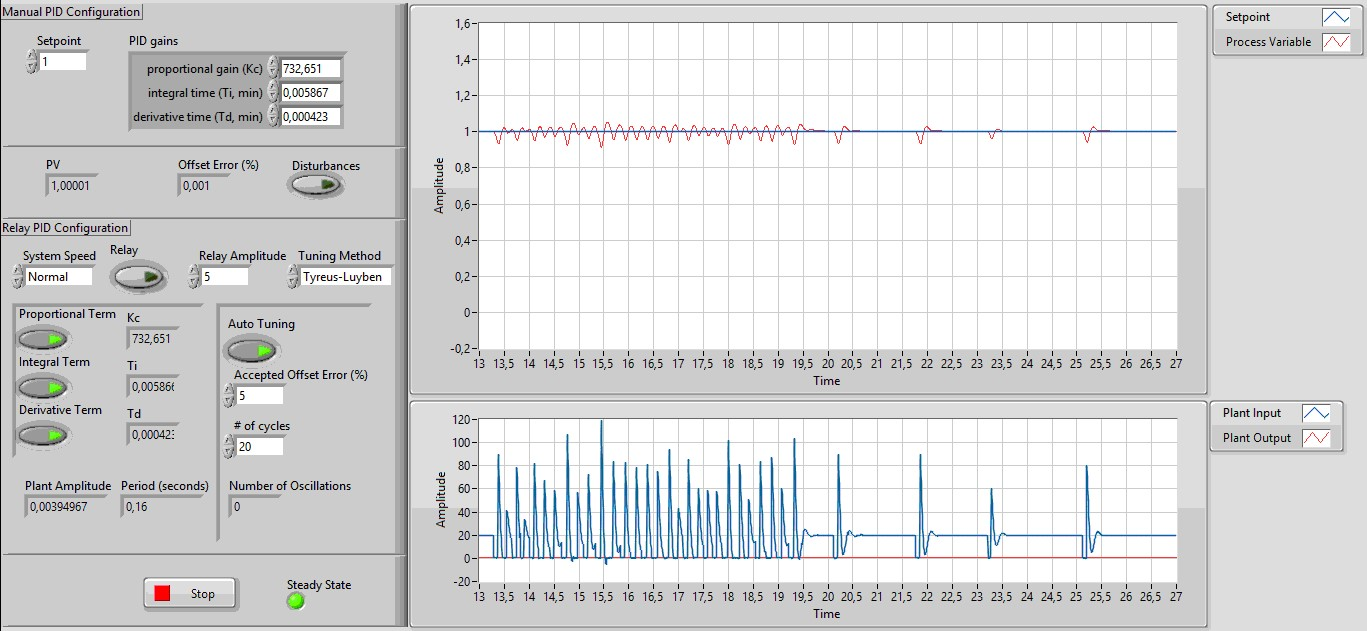
\includegraphics[width=\textwidth,height=5cm,keepaspectratio]{mass_spring_damper_disturbances_TL}
  \caption{Αντιμετώπιση διαταραχών του αυτο-ρυθμιζόμενου PID ελεγκτή του οποίου τα κέρδη έχουν υπολογιστεί με τους τύπους Tyreus-Luyben}
  \label{fig:mass_spring_damper_disturbances_TL}
\end{figure}

\subsection{Αποτελέσματα}

Στην ενότητα αυτή έγινε προσπάθεια να ελεγχθεί το κλασικό σύστημα ελέγχου που αποτελείται από μία μάζα, ένα ελατήριο και έναν αποσβεστήρα. Ως είσοδος του συστήματος θεωρήθηκε η δύναμη $F$ που ασκείται στη μάζα, ενώ ως έξοδος του συστήματος θεωρήθηκε η μετατόπιση $x$ που έχει η μάζα από το σημείο ισορροπίας της. 

Αρχικά, είδαμε ότι χωρίς έλεγχο το σύστημα δεν ανταποκρίνεται καλά καθώς έχει μεγάλο χρόνο ανύψωσης και μεγάλο σφάλμα μόνιμης κατάστασης. Έτσι στην αρχή χρησιμοποιήθηκε αναλογικός έλεγχος για τη μείωση του σφάλματος και τη βελτίωση του χρόνου ανύψωσης ο οποίος οδήγησε σε μία αξιοπρεπή απόκριση αλλά δεν κατάφερε να μηδενίσει το σφάλμα, παρά μόνο να το μειώσει σε ένα μικρό ποσοστό. 

Στη συνέχεια, χρησιμοποιήθηκε και ο ολοκληρωτικός όρος προκειμένου να μηδενιστεί το σφάλμα μόνιμης κατάστασης. Η τιμή του κέρδους όμως που υπολογίστηκε για τον ολοκληρωτικό όρο είχε σαν αποτέλεσμα να οδηγήσει το σύστημα σε μία μορφή αστάθειας. Αυτό οφείλεται στο ότι τόσο ο αναλογικός όσο και ο ολοκληρωτικός όρος μειώνουν το χρόνο ανύψωσης και ενισχύουν την υπερακόντιση του συστήματος οπότε προσθετικά οδηγούν την έξοδο του συστήματος σε ταλάντωση. Κανονικά, αν θα θέλαμε να έχουμε μόνο αναλογικό-ολοκληρωτικό έλεγχο θα έπρεπε, πριν την εφαρμογή του ολοκληρωτικού όρου, να μειώσουμε το αναλογικό κέρδος $K_c$. Όμως, στόχος μας στην παρούσα εργασία είναι να δούμε πόσο αποτελεσματικός είναι ο έλεγχος που παρέχει ο αυτο-ρυθμιζόμενος PID ελεγκτής που υλοποιήθηκε, χωρίς να πειράξουμε χειροκίνητα τα κέρδη που υπολογίζει.

Συνεπώς, για να βελτιώσουμε την απόκριση, προστέθηκε και ο διαφορικός όρος του ελεγκτή. Πλέον, ο έλεγχος που περιελάμβανε και τους τρεις όρους οδήγησε το σύστημα στο να έχει γρήγορο χρόνο ανύψωσης, μικρό ποσοστό υπερακόντισης και μηδενικό σφάλμα μόνιμης κατάστασης. Επίσης, αλλάζοντας την ταχύτητα που θέλουμε να έχει το κλειστό σύστημα ελέγχου ή επιλέγοντας τους τύπους Tyreus-Luyben αντί για τους Ziegler-Nichols, πετυχαίνουμε μια λιγότερο ``επιθετική" απόκριση. Παρόλο που είναι δύσκολο να πούμε ότι κάποιος έλεγχος είναι ξεκάθαρα καλύτερος από κάποιον άλλο αφού αυτό εξαρτάται από τις απαιτήσεις της κάθε διεργασίας, είναι ασφαλές να δηλώσουμε ότι τα κέρδη που υπολογίζονται με τους τύπους Tyreus-Luyben συνδυάζουν, ως ένα βαθμό, τις προηγούμενες αποκρίσεις, προσφέροντας έτσι τον περισσότερο ``σφαιρικό" έλεγχο.

\section{Σύστημα Cruise Control}

\subsection{Μαθηματικό Μοντέλο}

Το δεύτερο σύστημα που θα αναλυθεί είναι ένα πολύ καλό παράδειγμα ελέγχου ανάδρασης. Ο αυτόματος έλεγχος ταχύτητας ή \emph{cruise control} όπως είναι γνωστό στη διεθνή βιβλιογραφία, είναι ένα χαρακτηριστικό που βρίσκεται σε πολλά σύγχρονα αυτοκίνητα. Στόχος του είναι να κρατάει σταθερή την ταχύτητα του οχήματος, ανεξαρτήτως των διαταραχών που μπορεί να δέχεται από το περιβάλλον του, όπως η αντίσταση του ανέμου ή η κλίση του δρόμου. Αυτό το επιτυγχάνει μετρώντας την τρέχουσα ταχύτητα του οχήματος, συγκρίνοντας την με την επιθυμητή ταχύτητα και αυτόματα προσαρμόζοντας το γκάζι.

\begin{figure}[h]
  \centering
  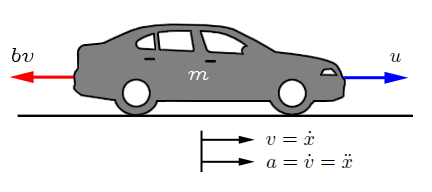
\includegraphics[width=\textwidth,height=5cm,keepaspectratio]{cruise_control_schematic}
  \caption{Μοντέλο συστήματος Αυτόματου Ελέγχου Ταχύτητας}
  \label{fig:cruise_control_schematic}
\end{figure}

Για την εύρεση των εξισώσεων του συστήματος, θεωρούμε ένα απλό μοντέλο της δυναμικής του οχήματος που φαίνεται στο παραπάνω διάγραμμα ελευθέρου σώματος. Το όχημα, μάζας $m$, ελέγχεται από μια δύναμη ελέγχου $u$. Η δύναμη αυτή αντιπροσωπεύει τη δύναμη που παράγεται στη διεπαφή δρόμου - ελαστικού. Για αυτό το απλοποιημένο μοντέλο, θα υποθέσουμε ότι μπορούμε να ελέγξουμε άμεσα αυτή τη δύναμη και θα παραμελήσουμε τη δυναμική του κινητήρα, των ελαστικών καθώς και των απωλειών που πηγαίνουν στη δημιουργία της δύναμης. Οι δυνάμεις αντίστασης, που οφείλονται στις τριβές των ελαστικών με το δρόμο και την αντίσταση του ανέμου, θεωρούμε ότι μεταβάλλονται γραμμικά με την ταχύτητα του οχήματος, $v$, και ενεργούν προς την αντίθετη κατεύθυνση από αυτή που κινείται το όχημα.

Με αυτές τις υποθέσεις, οδηγούμαστε σε ένα απλό σύστημα πρώτης τάξης. Αθροίζοντας τις δυνάμεις στον άξονα $x$ και εφαρμόζοντας τον $2^o$ Νόμο του Νεύτωνα, καταλήγουμε στην παρακάτω εξίσωση
\begin{equation}
m\dot{\upsilon} + b\upsilon = u
\label{eq:cruise_control_ode}
\end{equation}
όπου $u$ είναι η δύναμη που εφαρμόζεται στο όχημα και αποτελεί την είσοδο του συστήματος και $\upsilon$ είναι η ταχύτητα του οχήματος και αποτελεί την έξοδό του.

Παίρνοντας λοιπόν το μετασχηματισμό Laplace και στα δύο μέλη της εξίσωσης \ref{eq:cruise_control_ode} και θεωρώντας μηδενικές αρχικές συνθήκες, καταλήγουμε στη συνάρτηση μεταφοράς του συστήματος
\begin{equation}
P(s) = \frac{V(s)}{U(s)} = \frac{1}{ms+b} \left[\frac{m/s}{N}\right]
\label{eq:cruise_control_laplace}
\end{equation}

\subsection{Πείραμα}

Θεωρούμε ότι οι τιμές των παραμέτρων είναι $m = 1000\ kg$ και $\displaystyle b = 50\ \frac{Ns}{m}$. Με αντικατάσταση των τιμών στη συνάρτηση μεταφοράς έχουμε
\begin{equation}
\frac{V(s)}{U(s)} = \frac{1}{1000s+50}
\end{equation}

\subsubsection{Απόκριση Χωρίς Έλεγχο}

Αρχικά, ελέγχουμε να δούμε κατά πόσο το σύστημα χρειάζεται έλεγχο για να έχει ικανοποιητική απόδοση. Η απόκριση του συστήματος σε μια είσοδο βαθμίδας μοναδιαίου πλάτους φαίνεται στο παρακάτω σχήμα.

\begin{figure}[h]
  \centering
  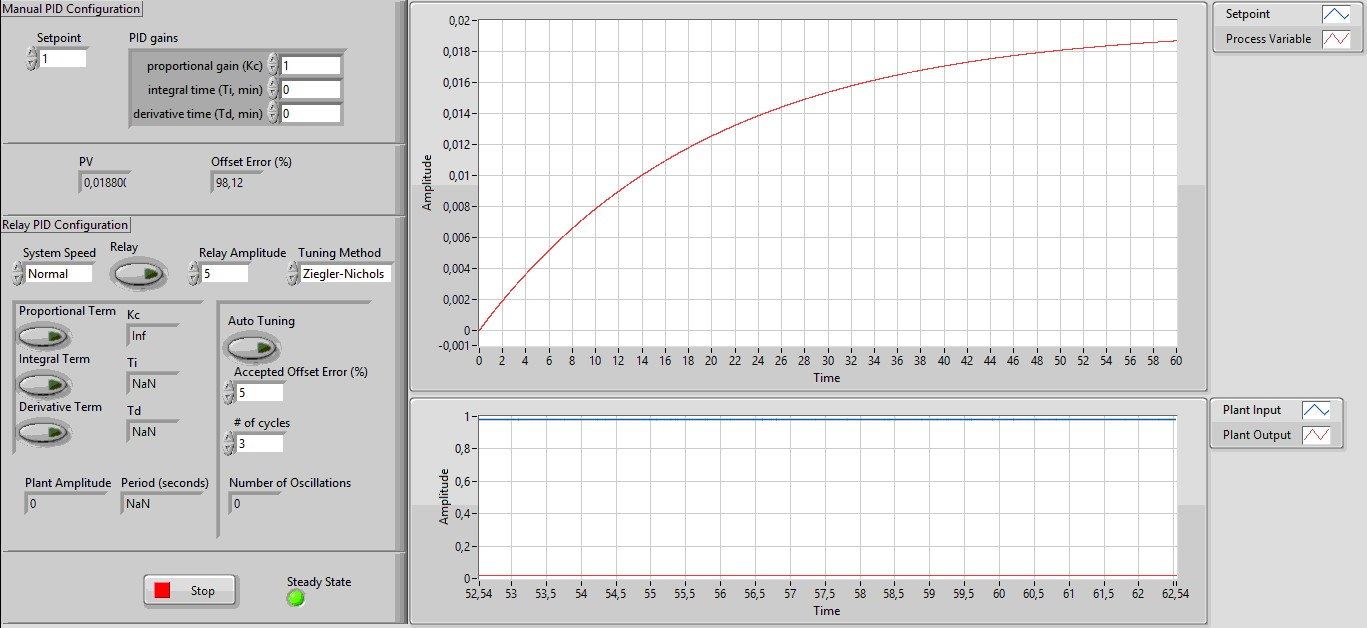
\includegraphics[width=\textwidth,height=5cm,keepaspectratio]{cruise_control_no_control}
  \caption{Βηματική απόκριση του συστήματος Αυτόματου Ελέγχου Ταχύτητας}
  \label{fig:cruise_control_no_control}
\end{figure}

Από την γραφική παράσταση βλέπουμε ότι η απόκριση του συστήματος χωρίς έλεγχο είναι πολύ αργή και έχει πολύ μεγάλο σφάλμα μόνιμης κατάστασης. 

%\subsubsection{Ταλαντώσεις του συστήματος}
%
%Επειδή το συγκεκριμένο σύστημα είναι πρώτης τάξεως, οι ταλαντώσεις που εκτελεί κατά το πείραμα relay, έχουν πολύ μικρό πλάτος και μικρή περίοδο. Το Σχήμα \ref{fig:cruise_control_oscillations} είναι η μεγέθυνση της απόκρισης του συστήματος έτσι ώστε να φανεί το πλάτος και η περίοδος των ταλαντώσεων αυτών. 
%
%\begin{figure}[h]
%  \centering
%  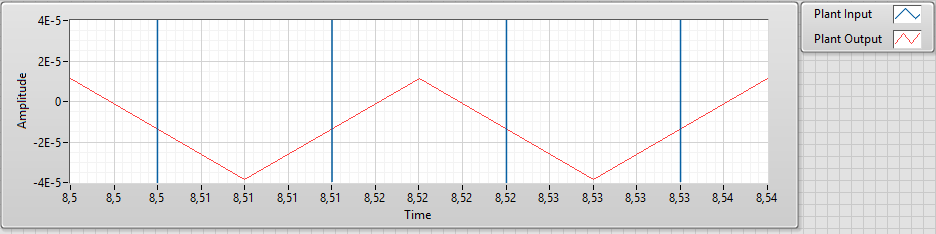
\includegraphics[width=\textwidth,height=5cm,keepaspectratio]{cruise_control_oscillations}
%  \caption{Ταλαντώσεις του συστήματος Αυτομάτου Ελέγχου Ταχύτητας}
%  \label{fig:cruise_control_oscillations}
%\end{figure}

\subsubsection{Αναλογικός Έλεγχος}

Στο Σχήμα \ref{fig:cruise_control_proportional} φαίνεται η απόκριση του συστήματος όταν ο PID ελεγκτής χρησιμοποιεί μόνο τον αναλογικό του όρο. Βλέπουμε ότι για το κέρδος του αναλογικού όρου έχει υπολογιστεί μια υπερβολικά μεγάλη τιμή, συγκεκριμένα $K_c = 176463$. Πέρα από αυτό, η απόκριση του συστήματος πλέον έχει βελτιωθεί καθώς φτάνει στο επιθυμητό σημείο σε περίπου έξι δευτερόλεπτα και το σφάλμα μόνιμης κατάστασης έχει πλέον τιμή $0.028\%$.

\begin{figure}[h]
  \centering
  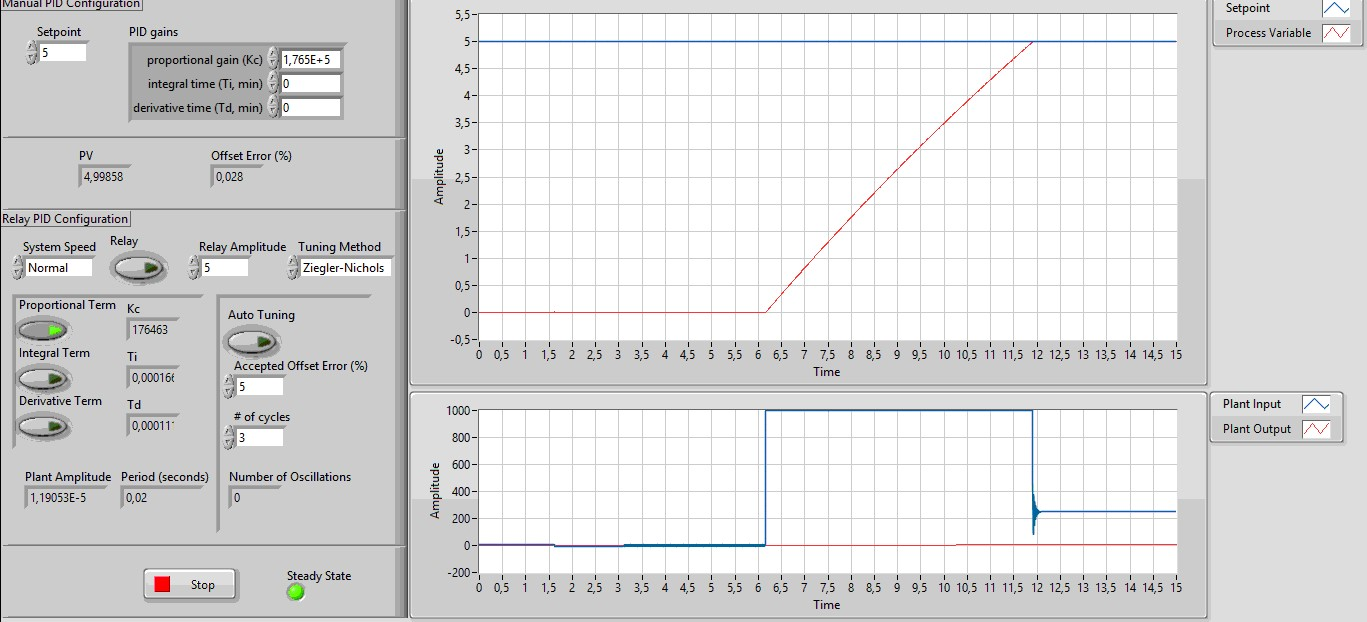
\includegraphics[width=\textwidth,height=5cm,keepaspectratio]{cruise_control_proportional}
  \caption{Βηματική απόκριση του συστήματος Αυτομάτου Ελέγχου Ταχύτητας με χρήση μόνο του αναλογικού όρου}
  \label{fig:cruise_control_proportional}
\end{figure}

\subsubsection{Αναλογικός - Ολοκληρωτικός Έλεγχος}

Στο Σχήμα \ref{fig:cruise_control_integral} φαίνεται η βηματική απόκριση του συστήματος όταν στον έλεγχο προστεθεί και ο ολοκληρωτικός όρος. Τόσο αυτή η απόκριση όσο και η προηγούμενη παρουσιάζουν πολλές ομοιότητες. Ο χρόνος ανύψωσης είναι σχεδόν ίδιος και η έξοδος του συστήματος έχει γραμμική μεταβολή συναρτήσει του χρόνου. Το μόνο που διαφέρει σε σχέση με πριν είναι ότι πλέον, λόγω του ολοκληρωτικού όρου, το σφάλμα μόνιμης κατάστασης είναι εντελώς μηδέν.

\begin{figure}[h]
  \centering
  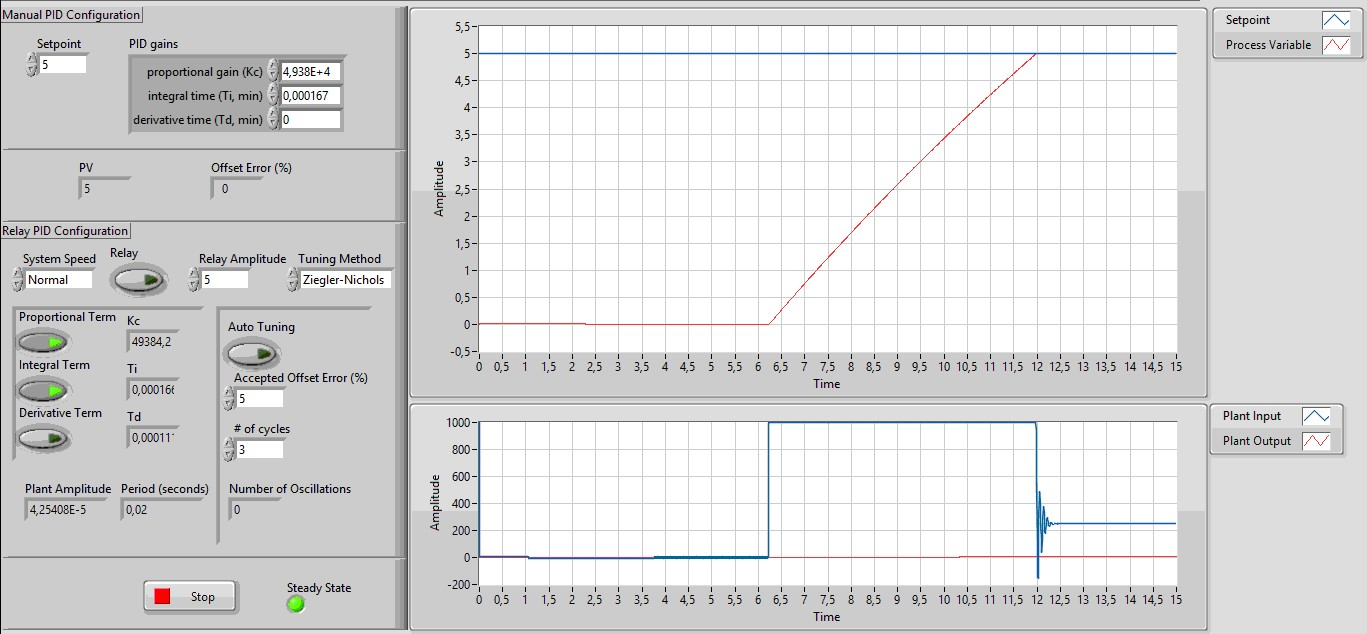
\includegraphics[width=\textwidth,height=5cm,keepaspectratio]{cruise_control_integral}
  \caption{Βηματική απόκριση του συστήματος Αυτομάτου Ελέγχου Ταχύτητας με χρήση του αναλογικού και του ολοκληρωτικού όρου}
  \label{fig:cruise_control_integral}
\end{figure}

\subsubsection{Αναλογικός - Ολοκληρωτικός - Διαφορικός Έλεγχος}

Στο Σχήμα \ref{fig:cruise_control_derivative} φαίνεται η απόκριση του συστήματος όταν ο ελεγκτής χρησιμοποιεί και τους τρεις όρους του. Από τη γραφική παράσταση εύκολα βγαίνει το συμπέρασμα ότι η απόκριση δεν άλλαξε καθόλου με την προσθήκη του διαφορικού όρου.

\begin{figure}[h]
  \centering
  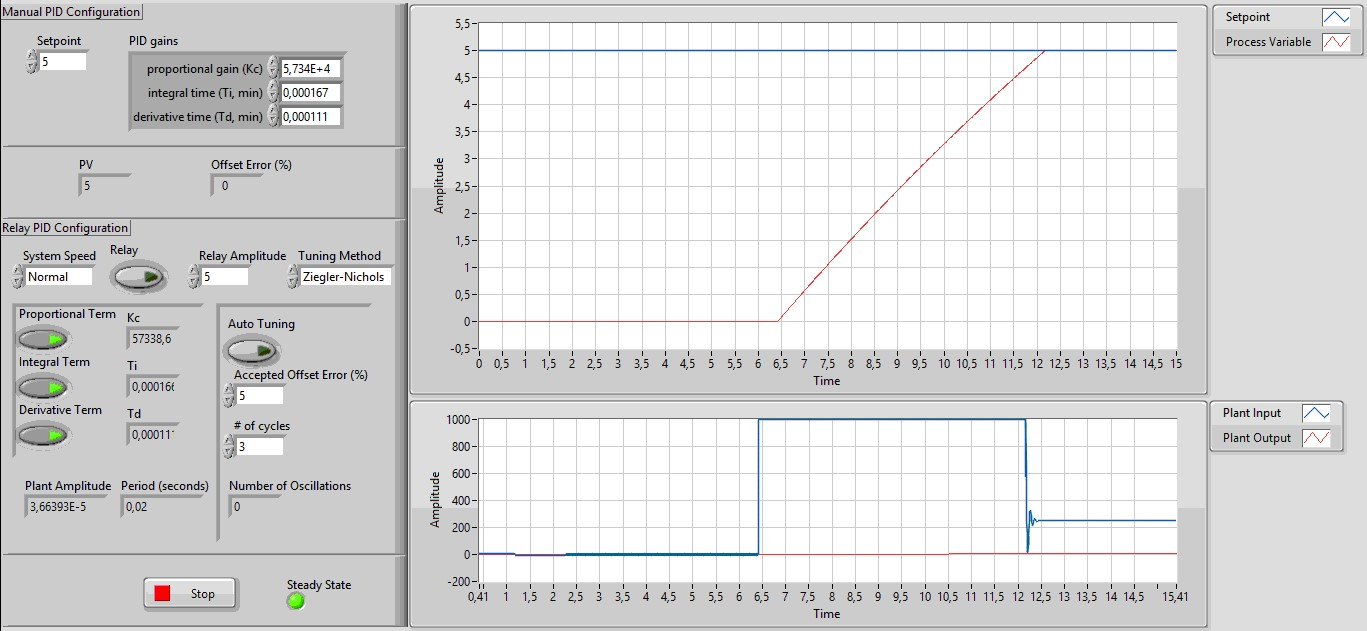
\includegraphics[width=\textwidth,height=5cm,keepaspectratio]{cruise_control_derivative}
  \caption{Βηματική απόκριση του συστήματος Αυτομάτου Ελέγχου Ταχύτητας με χρήση και των τριών όρων του PID ελεγκτή}
  \label{fig:cruise_control_derivative}
\end{figure}

Τέλος, στο Σχήμα \ref{fig:cruise_control_TL} φαίνεται η απόκριση του συστήματος όταν για τον αυτόματο υπολογισμό των κερδών του αναλογικού και του ολοκληρωτικού όρου έχουν χρησιμοποιηθεί οι τύποι Tyreus-Luyben. Όπως ήταν αναμενόμενο, ούτε σε αυτή την περίπτωση η απόκριση του συστήματος παρουσιάζει αλλαγές σε σχέση με τις προηγούμενες γραφικές παραστάσεις.

\begin{figure}[h]
  \centering
  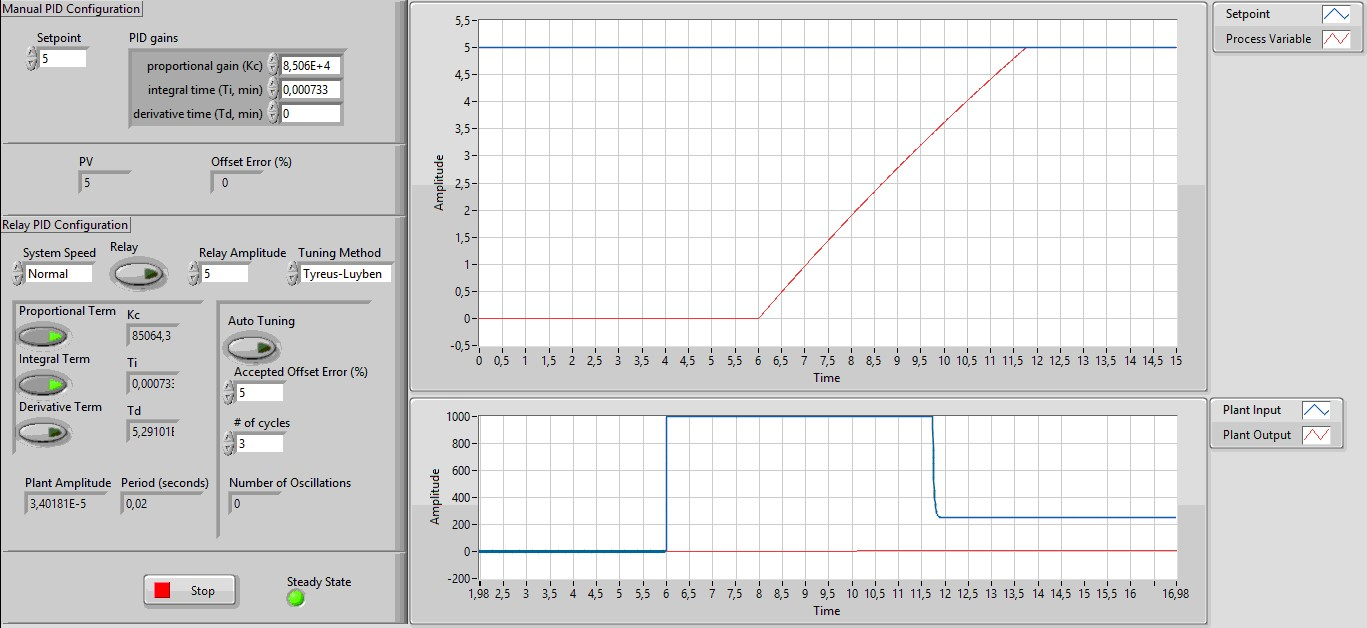
\includegraphics[width=\textwidth,height=5cm,keepaspectratio]{cruise_control_TL}
  \caption{Βηματική απόκριση του συστήματος Αυτομάτου Ελέγχου Ταχύτητας με χρήση και των τριών όρων του PID ελεγκτή όπου τα κέρδη έχουν υπολογιστεί χρησιμοποιώντας τους τύπους Tyreus-Luyben}
  \label{fig:cruise_control_TL}
\end{figure}

\subsubsection{Αντιμετώπιση Διαταραχών}

Αφού από τα διαδοχικά πειράματα καταλήξαμε στο συμπέρασμα ότι οι αποκρίσεις δεν έχουν αλλαγές μεταξύ τους, ο πιο ικανοποιητικός έλεγχος θα μπορούσαμε να πούμε ότι είναι αυτός που δεν περιλαμβάνει το διαφορικό όρο, καθώς δεν προσφέρει κάτι παραπάνω. 

Στα σχήματα \ref{fig:cruise_control_disturbances} και \ref{fig:cruise_control_disturbances_TL} φαίνεται πώς το κλειστό σύστημα αποκρίνεται στις ξαφνικές διαταραχές που εισέρχονται στο βρόχο ελέγχου. Και σε αυτή την περίπτωση, οι δύο γραφικές παραστάσεις μοιάζουν υπερβολικά πολύ. Παρόλα αυτά, οι διαταραχές αντιμετωπίζονται ικανοποιητικά και το σύστημα επιστρέφει στην επιθυμητή τιμή μετά το πέρας αυτών. 

\begin{figure}[h]
  \centering
  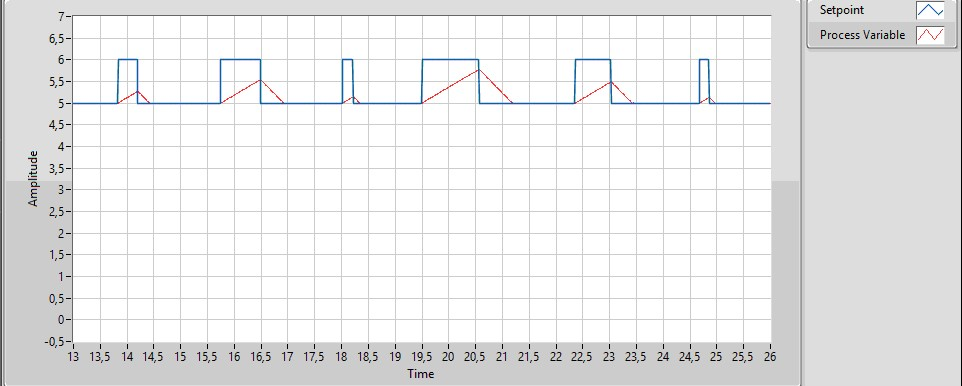
\includegraphics[width=\textwidth,height=5cm,keepaspectratio]{cruise_control_disturbances}
  \caption{Αντιμετώπιση διαταραχών του αυτο-ρυθμιζόμενου PID ελεγκτή του οποίου τα κέρδη έχουν υπολογιστεί με τους τύπους Ziegler-Nichols}
  \label{fig:cruise_control_disturbances}
\end{figure}

\begin{figure}[h]
  \centering
  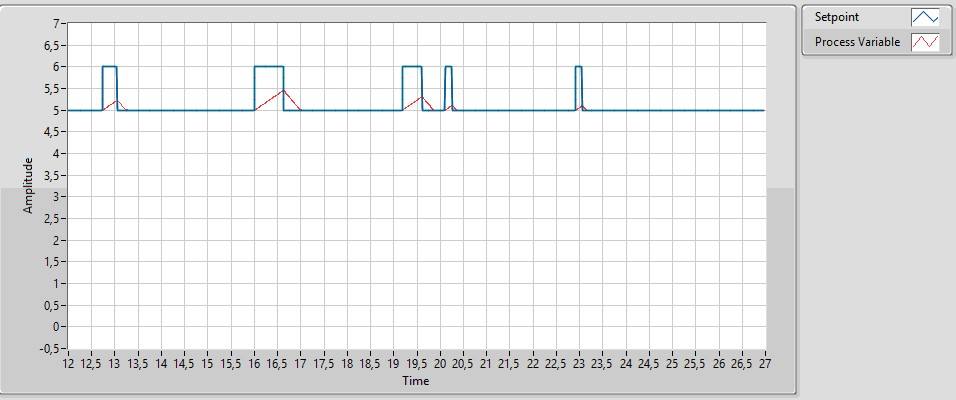
\includegraphics[width=\textwidth,height=5cm,keepaspectratio]{cruise_control_disturbances_TL}
  \caption{Αντιμετώπιση διαταραχών του αυτο-ρυθμιζόμενου PID ελεγκτή του οποίου τα κέρδη έχουν υπολογιστεί με τους τύπους Tyreus-Luyben}
  \label{fig:cruise_control_disturbances_TL}
\end{figure}

\subsection{Αποτελέσματα}

Σε αυτή την ενότητα έγινε προσπάθεια να ελεγχθεί ένα σύστημα που συναντάται σε καθημερινή βάση σε όλα τα σύγχρονα οχήματα. Αρχικά, με μία απλή προσομοίωση κατέστη εμφανές ότι το σύστημα χρήζει ελέγχου, αφού χωρίς ελεγκτή η απόκριση ήταν πολύ αργή και η έξοδος του συστήματος είχε τιμή περίπου $y(t) = 0.02$ αντί για $y(t) = 1$ που ήταν το επιθυμητό. Αυτό είναι λογικό, αφού η συνάρτηση μεταφοράς (Εξίσωση \ref{eq:cruise_control_laplace}) για τις δοθείσες τιμές των παραμέτρων έχει κέρδος ανοιχτού βρόχου $\displaystyle \frac{1}{50} = 0.02$.

Προχωρώντας λοιπόν στον έλεγχο του συστήματος παρατηρήθηκε κάτι αρκετά ενδιαφέρον. Ασχέτως με τον τύπο ελέγχου που χρησιμοποιήθηκε ή τη μέθοδο με την οποία υπολογίστηκαν τα κέρδη, η απόκριση του κλειστού συστήματος φαίνεται να μένει ανεπηρέαστη. Αυτό αποτελεί ένα εν γένει χαρακτηριστικό του εν λόγω συστήματος και στον τρόπο που έχει μοντελοποιηθεί. Το συγκεκριμένο σύστημα είναι ένα αμάξι που πρέπει να διατηρεί σταθερή ταχύτητα. Όπως είναι φυσικό, η μάζα του οχήματος έχει μεγάλη τιμή, $m = 1000\ kg$ στο συγκεκριμένο παράδειγμα. Αυτό συνεπάγεται ότι ο έλεγχος θα πρέπει να έχει πολύ μεγάλη τιμή προκειμένου να προκαλέσει τις επιθυμητές αλλαγές στην ταχύτητα του αμαξιού.

Σε μια πραγματική εφαρμογή, στην οποία υπάρχουν περιορισμοί λόγω των φυσικών ορίων των συσκευών που χρησιμοποιούνται, η τιμή του ελέγχου θα πρέπει να περιορίζεται έτσι ώστε να αποφεύγεται η ταλαιπωρία και ενδεχομένως και η καταστροφή του εξοπλισμού. Στην εργασία αυτή, για την προσομοίωση ενός πραγματικού συστήματος ελέγχου, η έξοδος του ελεγκτή δεν μπορεί να ξεπερνάει τις τιμές $1000$ και $-1000$. Συνεπώς, στο συγκεκριμένο σύστημα ελέγχου, λόγω της μεγάλης μάζας του οχήματος, η έξοδος του ελεγκτή έρχεται σε κορεσμό, οποιοδήποτε είδος ελέγχου και να χρησιμοποιείται. Αυτό φαίνεται στα σχήματα \ref{fig:cruise_control_proportional}, \ref{fig:cruise_control_integral}, \ref{fig:cruise_control_derivative} και \ref{fig:cruise_control_TL} στη κάτω γραφική παράσταση που δείχνει την είσοδο του συστήματος (έξοδος του ελεγκτή) σε σχέση με την έξοδο του συστήματος. Έτσι λοιπόν εξηγείται γιατί το σύστημα έχει παρόμοια απόκριση ανεξαρτήτως του ελέγχου που χρησιμοποιείται. 

Ενδεικτικά, στο Σχήμα \ref{fig:cruise_control_no_limits} φαίνεται η θεωρητική απόκριση που θα είχε το σύστημα αν δεν υπήρχαν τα προαναφερθέντα όρια στην έξοδο του ελεγκτή και για αναλογικό κέρδος $K_c = 5000$. Εύκολα παρατηρούμε ότι η απόκριση είναι πολύ διαφορετική από αυτές που είδαμε προηγουμένως. Το σύστημα χρειάζεται μόνο μισό δευτερόλεπτο για να φτάσει στο $90\%$ της τελικής τιμής του σε αντίθεση με τα περίπου έξι δευτερόλεπτα που χρειαζόταν όταν το σήμα ελέγχου περιοριζόταν. Αυτό βέβαια για να επιτευχθεί χρειάζεται μια τεράστια τιμή ελέγχου, συγκεκριμένα η τιμή αυτή για τη δοθείσα τιμή του αναλογικού κέρδους είναι $controller\ output = 50000$. Όπως εξηγήθηκε, μια τέτοια τιμή σε ένα πραγματικό σύστημα θα μπορούσε να έχει ολέθριες συνέπειες για τον εξοπλισμό, συνεπώς μια τέτοια απόκριση παραμένει πραγματοποιήσιμη μόνο σε θεωρητικό επίπεδο.

\begin{figure}[h]
  \centering
  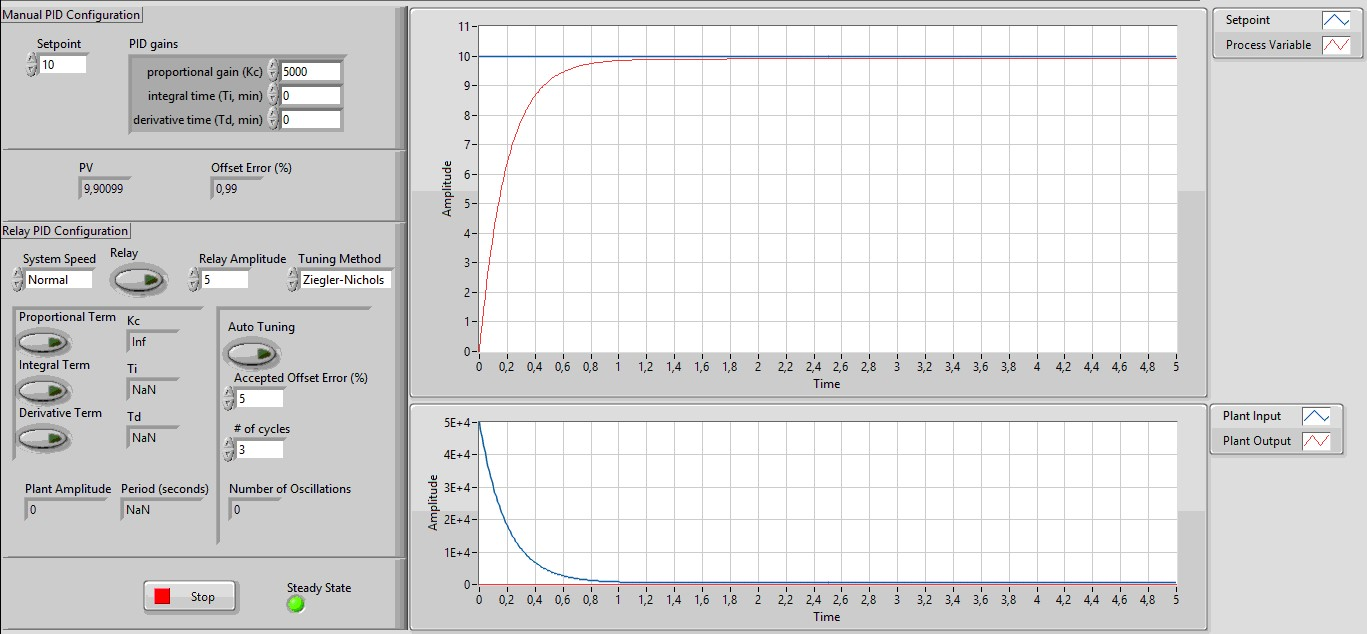
\includegraphics[width=\textwidth,height=5cm,keepaspectratio]{cruise_control_no_limits}
  \caption{Βηματική απόκριση του συστήματος Αυτόματου Ελέγχου Ταχύτητας χωρίς όριο για την έξοδο του ελεγκτή}
  \label{fig:cruise_control_no_limits}
\end{figure}

Επειδή το σύστημα είναι πρώτης τάξης, οι ταλαντώσεις που εκτελεί κατά τη διαδικασία ρύθμισης έχουν πολύ μικρό πλάτος και περίοδο με αποτέλεσμα τα κέρδη που υπολογίζονται να είναι πολύ υψηλά. Αυτό όμως εν τέλει δεν επηρεάζει την απόκριση του συστήματος καθώς η έξοδος του ελεγκτή λειτουργεί μέσα σε συγκεκριμένες τιμές. Συνοψίζοντας, δεδομένου των περιορισμών που αναφέρθηκαν, ο αυτο-ρυθμιζόμενος ελεγκτής προσφέρει μια αρκετά ικανοποιητική μορφή ελέγχου.

\section{Σύστημα Motor Speed}

\subsection{Μαθηματικό Μοντέλο}

Ένας κοινός ενεργοποιητής στα συστήματα ελέγχου είναι ο DC κινητήρας (\emph{κινητήρας συνεχούς ρεύματος}). Αυτός παρέχει άμεσα περιστροφική κίνηση και σε συνδυασμό με με τροχούς και άλλα μέσα μπορεί να προσφέρει και μεταφορική κίνηση. Το ηλεκτρικό ισοδύναμο ενός  DC κινητήρα και το διάγραμμα ελευθέρου σώματος φαίνονται στο παρακάτω σχήμα. 

\begin{figure}[h]
  \centering
  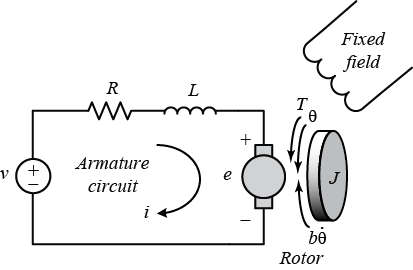
\includegraphics[width=\textwidth,height=5cm,keepaspectratio]{motor}
  \caption{Μοντέλο συστήματος ενός DC κινητήρα}
  \label{fig:motor}
\end{figure}

Για αυτό το παράδειγμα, θα θεωρήσουμε ότι η είσοδος του συστήματος είναι η τάση $V$ που εφαρμόζεται στο κύκλωμα και η έξοδος είναι η γωνιακή ταχύτητα $\dot{\theta}$ του άξονα. Ο ρότορας και ο άξονας υποτίθεται ότι είναι άκαμπτοι. Επίσης υποθέτουμε ότι η ροπή τριβής είναι ανάλογη της γωνιακής ταχύτητας του άξονα.

Γενικά, η ροπή που παράγεται από έναν κινητήρα συνεχούς ρεύματος είναι ανάλογη προς το ρεύμα οπλισμού και τη δύναμη του μαγνητικού πεδίου. Σε αυτό το παράδειγμα, θα υποθέσουμε ότι το μαγνητικό πεδίο είναι σταθερό και, συνεπώς, ότι η ροπή του κινητήρα είναι ανάλογη μόνο προς το ρεύμα $i$ του οπλισμού κατά ένα σταθερό παράγοντα $K_t$ όπως φαίνεται στην παρακάτω εξίσωση. Αυτό αναφέρεται ως κινητήρας ελεγχόμενος από οπλισμό.
\begin{equation}
T = K_ti
\end{equation}
Η πίσω ηλεκτροκινητική δύναμη (\emph{back emf}), $e$, είναι ανάλογη της γωνιακής ταχύτητας του άξονα με σταθερό παράγοντα $K_e$.
\begin{equation}
e = K_e\dot{\theta}
\end{equation}
Σε μονάδες SI, οι σταθερές του κινητήρα και της πίσω ηλεκτροκινητικής δύναμης είναι ίσες, δηλαδή, $K_t = K_e$. Ως εκ τούτου, θα χρησιμοποιήσουμε τη σταθερά $K$ για να αντιπροσωπεύσουμε τόσο τη σταθερά της ροπής του κινητήρα όσο και την σταθερά της πίσω ηλεκτροκινητικής δύναμης. Από το Σχήμα \ref{fig:motor}, μπορούμε να βρούμε τις ακόλουθες εξισώσεις που βασίζονται στον $2^o$ νόμο του Νεύτωνα και στον νόμο περί τάσης του Kirchhoff.
\begin{equation}
J\ddot{\theta} + b\dot{\theta} = Ki
\end{equation}
\begin{equation}
L\frac{di}{dt} + Ri = V - K\dot{\theta}
\end{equation}
Εφαρμόζοντας το μετασχηματισμό Laplace, οι παραπάνω εξισώσεις μοντελοποίησης μπορούν να εκφραστούν με τη μεταβλητή Laplace $s$.
\begin{equation}
s(Js+b)\Theta(s) = KI(s)
\end{equation}
\begin{equation}
(Ls+R)I(s) = V(s) - Ks\Theta(s)
\end{equation}
Εξαλείφοντας τον όρο $I(s)$ από τις δύο παραπάνω εξισώσεις καταλήγουμε στην ακόλουθη συνάρτηση μεταφοράς ανοιχτού συστήματος, όπου η γωνιακή ταχύτητα θεωρείται η έξοδος και η τάση θεωρείται η είσοδος
\begin{equation}
P(s) = \frac{\dot{\Theta}}{V(s)} = \frac{K}{(JL)s^2+(RJ+bL)s+(bR+K^2)} \left[\frac{rad/sec}{V}\right]
\label{eq:motor_laplace}
\end{equation}

\subsection{Πείραμα}

Για το παράδειγμα αυτό θεωρούμε ότι οι τιμές των παραμέτρων είναι ως εξής
\begin{flushleft}
\begin{tabular}{lll}
\textbf{J} & ροπή αδράνειας του ρότορα & $0.01\ kgm^2$ \\ 
\textbf{b} & σταθερά τριβής & $0.1\ Nms$ \\  
$\mathbf{K_e}$ & σταθερά ηλεκτροκινητικής δύναμης & $0.01\ \frac{V}{rad/sec}$ \\  
$\mathbf{K_t}$ & σταθερά ροπής του κινητήρα & $0.01\ \frac{Nm}{Ampere}$ \\  
\textbf{R} & ηλεκτρική αντίσταση & $1\ Ohm$ \\ 
\textbf{L} & ηλεκτρική επαγωγή & $0.5\ H$ \\ 
\end{tabular} 
\end{flushleft}

Αντικαθιστώντας τις τιμές αυτές στη σχέση \ref{eq:motor_laplace} έχουμε την παρακάτω εξίσωση
\begin{equation}
P_{motor} = \frac{0.01}{0.005s^2+0.06s+0.1001}
\end{equation}

\subsubsection{Απόκριση Χωρίς Έλεγχο}

Όπως και για τα προηγούμενα συστήματα, πρώτα δοκιμάζουμε την απόκριση του συστήματος όταν αυτό δουλεύει χωρίς έλεγχο.
\begin{figure}[h]
  \centering
  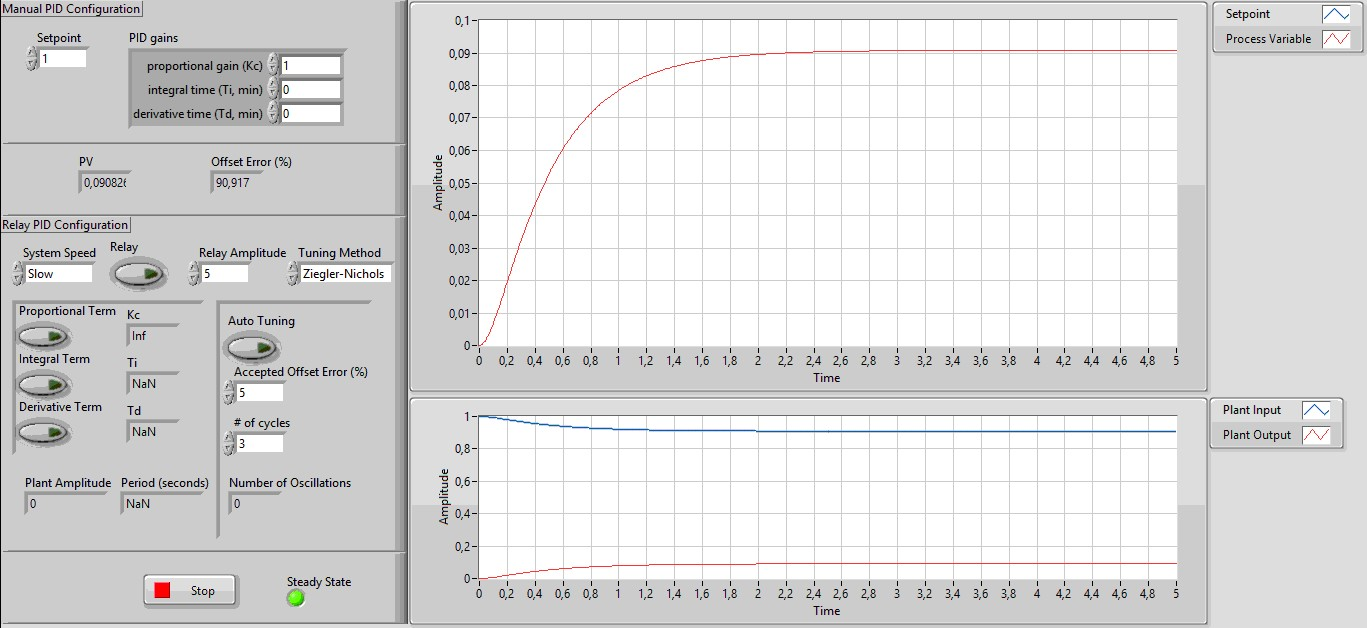
\includegraphics[width=\textwidth,height=5cm,keepaspectratio]{motor_no_control}
  \caption{Βηματική απόκριση του συστήματος ενός DC κινητήρα}
  \label{fig:motor_no_control}
\end{figure}
Από το παραπάνω σχήμα γίνεται εύκολα αντιληπτό ότι όταν το σύστημα λειτουργεί χωρίς έλεγχο η απόκριση του είναι κακή. Πιο συγκεκριμένα, βλέπουμε ότι για τάση εισόδου $1$ Volt, ο ρότορας στρέφεται με γωνιακή ταχύτητα $0.1\ \text{rad/sec}$ δηλαδή έχει δέκα φορές μικρότερη ταχύτητα από την επιθυμητή. Επίσης έχει χρόνο ανύψωσης περίπου δύο δευτερόλεπτα.

Επειδή το κυρίως ζητούμενο από ένα τέτοιο σύστημα είναι να περιστρέφεται στην επιθυμητή ταχύτητα, ο έλεγχος που θα εφαρμοστεί θέλουμε να έχει μικρό σφάλμα, μικρότερο από $1\%$. Άλλη απαίτηση ελέγχου είναι να έχει μικρό χρόνο ανύψωσης, έτσι ώστε να φτάνει σε σύντομο χρονικό διάστημα το επιθυμητό σημείο. Τέλος, λόγω του ότι η λειτουργία του κινητήρα σε ταχύτητα μεγαλύτερη της επιθυμητής μπορεί να δημιουργήσει προβλήματα στον εξοπλισμό, θέλουμε να έχει μικρό ποσοστό υπερακόντισης.

\subsubsection{Αναλογικός Έλεγχος}

Στο Σχήμα \ref{fig:motor_proportional} φαίνεται πώς συμπεριφέρεται το σύστημα όταν σε αυτό εφαρμόζεται μόνο αναλογικός έλεγχος, το κέρδος του οποίου έχει υπολογιστεί με τους τύπους Ziegler-Nichols και η ταχύτητα απόκρισης του συστήματος έχει οριστεί στο ``Normal". Αμέσως γίνεται εμφανές ότι το σύστημα ενώ έχει ικανοποιητικό χρόνο ανύψωσης, παρουσιάζει μεγάλο ποσοστό υπερακόντισης και εκτεταμένες ταλαντώσεις μέχρι να βρεθεί σε κατάσταση ισορροπίας.

\begin{figure}[h]
  \centering
  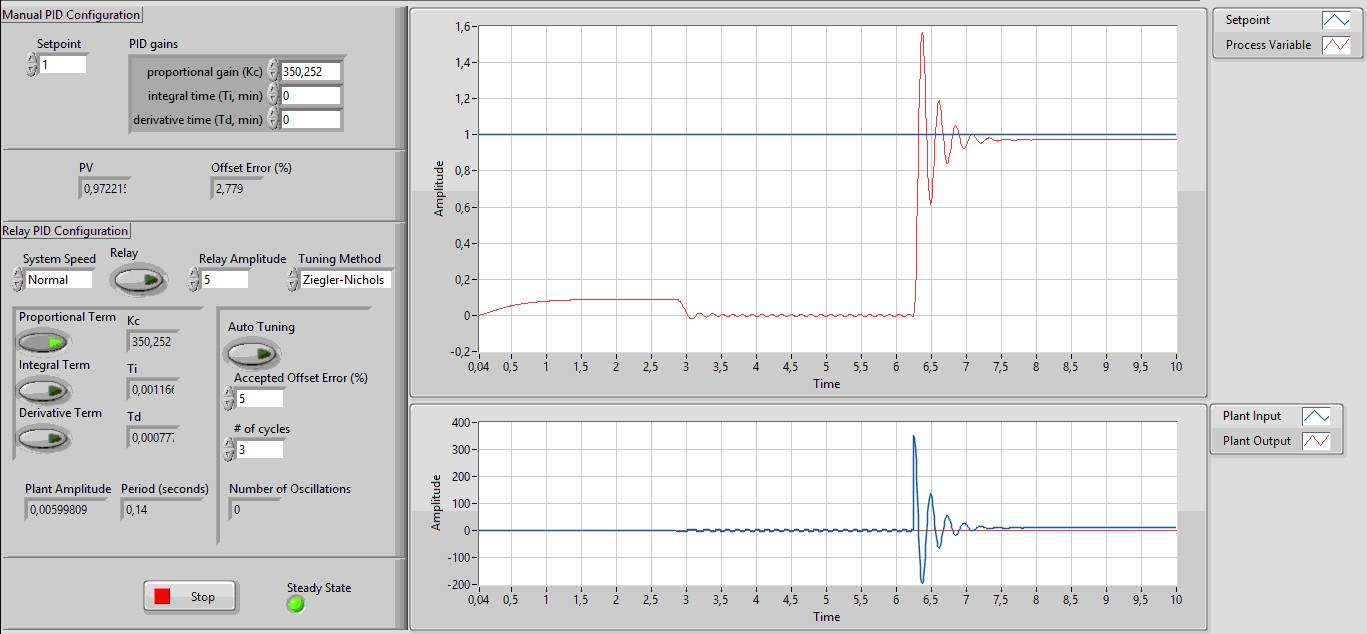
\includegraphics[width=\textwidth,height=5cm,keepaspectratio]{motor_proportional}
  \caption{Βηματική απόκριση του συστήματος ενός DC κινητήρα με εφαρμογή αναλογικού ελέγχου}
  \label{fig:motor_proportional}
\end{figure}

Στο Σχήμα \ref{fig:motor_proportional_slow} φαίνεται ότι όταν η επιθυμητή ταχύτητα απόκρισης οριστεί στο ``Slow" τόσο οι ταλαντώσεις όσο και η υπερακόντιση μειώνονται. Συνεπώς για τη συνέχεια του πειράματος αυτή θα είναι η λειτουργία που θα χρησιμοποιηθεί.

\begin{figure}[h]
  \centering
  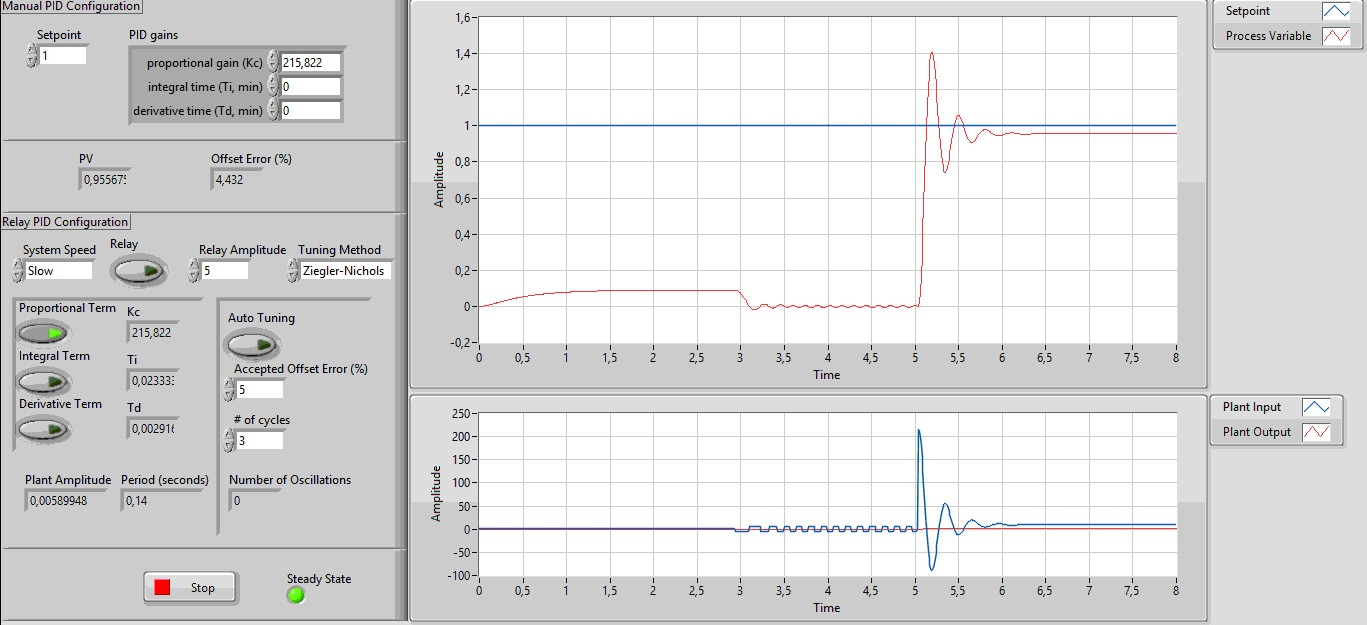
\includegraphics[width=\textwidth,height=5cm,keepaspectratio]{motor_proportional_slow}
  \caption{Βηματική απόκριση του συστήματος ενός DC κινητήρα με εφαρμογή αναλογικού ελέγχου και επιθυμητή ταχύτητα απόκρισης ``Slow"}
  \label{fig:motor_proportional_slow}
\end{figure}

\subsubsection{Αναλογικός - Διαφορικός Έλεγχος}

Συνεχίζοντας την προσπάθεια ελέγχου του συστήματος, προσθέτουμε και τον διαφορικό όρο. Το μεγαλύτερο πρόβλημα της προηγούμενης απόκρισης ήταν η μεταβατική κατάσταση του κινητήρα η οποία παρουσίαζε υψηλή υπερακόντιση και ταλαντώσεις. Για την αντιμετώπιση αυτών των φαινόμενων εισάγεται και ο διαφορικός έλεγχος. Η απόκριση του συστήματος παρουσιάζεται στο Σχήμα \ref{fig:motor_derivative_slow}.

Είναι εμφανές ότι ο διαφορικός όρος εξομάλυνε τη συμπεριφορά του συστήματος αλλά, όπως αναμενόταν, δεν μείωσε το σφάλμα μόνιμης κατάστασης το οποίο παραμένει στα ίδια επίπεδα με πριν.

\begin{figure}[h]
  \centering
  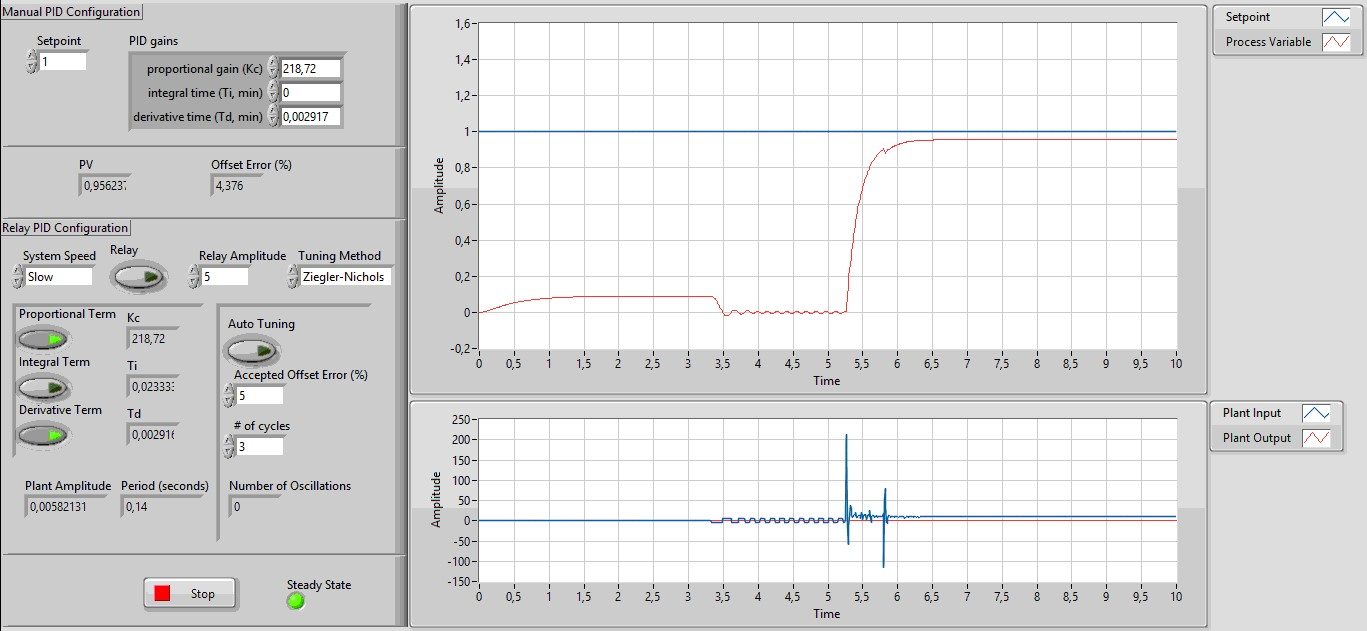
\includegraphics[width=\textwidth,height=5cm,keepaspectratio]{motor_derivative_slow}
  \caption{Βηματική απόκριση του συστήματος ενός DC κινητήρα με εφαρμογή αναλογικού - διαφορικού ελέγχου και επιθυμητή ταχύτητα απόκρισης ``Slow"}
  \label{fig:motor_derivative_slow}
\end{figure}

\subsubsection{Αναλογικός - Ολοκληρωτικός - Διαφορικός Έλεγχος}

Από τη γραφική παράσταση που φαίνεται στο Σχήμα \ref{fig:motor_pid_slow} βλέπουμε ότι πλέον έχουν εξομαλυνθεί τα αρνητικά χαρακτηριστικά της μεταβατικής κατάστασης και το μόνιμο σφάλμα είναι μηδενικό.

\begin{figure}[h]
  \centering
  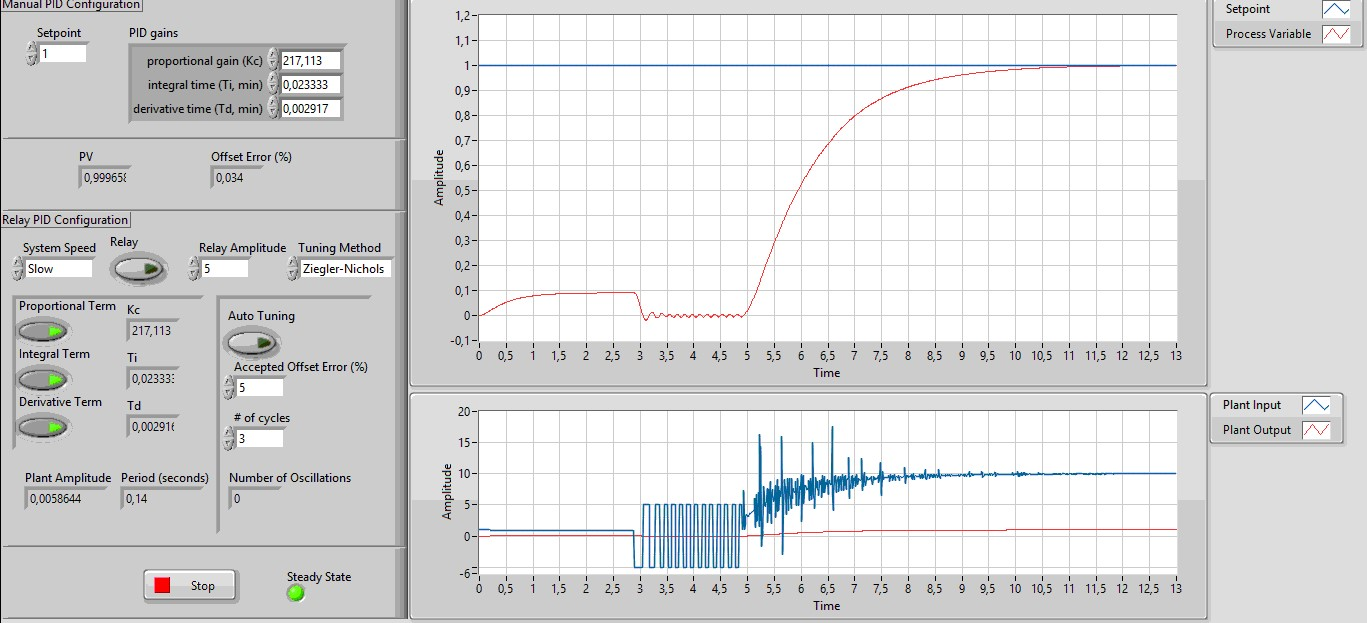
\includegraphics[width=\textwidth,height=5cm,keepaspectratio]{motor_pid_slow}
  \caption{Βηματική απόκριση του συστήματος ενός DC κινητήρα με εφαρμογή αναλογικού - ολοκληρωτικού - διαφορικού ελέγχου και επιθυμητή ταχύτητα απόκρισης ``Slow"}
  \label{fig:motor_pid_slow}
\end{figure}

Επίσης, η απόκριση του κινητήρα όταν αυτός ξεκινάει από την ηρεμία φαίνεται στο Σχήμα \ref{fig:motor_pid_slow_start}. Βλέπουμε ότι αυτή η απόκριση διαφέρει λίγο από την απόκριση που έχει ο κινητήρας όταν τη θέση του relay στοιχείου παίρνει ο ελεγκτής. Αυτό οφείλεται στις διαφορετικές αρχικές συνθήκες που υπάρχουν στο σύστημα. Όταν αυτό ξεκινάει από την ηρεμία οι αρχικές του συνθήκες είναι μηδενικές, ενώ όταν υπόκειται στο πείραμα για τον υπολογισμό των κερδών του αυτό φυσικά δεν ισχύει.

\begin{figure}[h]
  \centering
  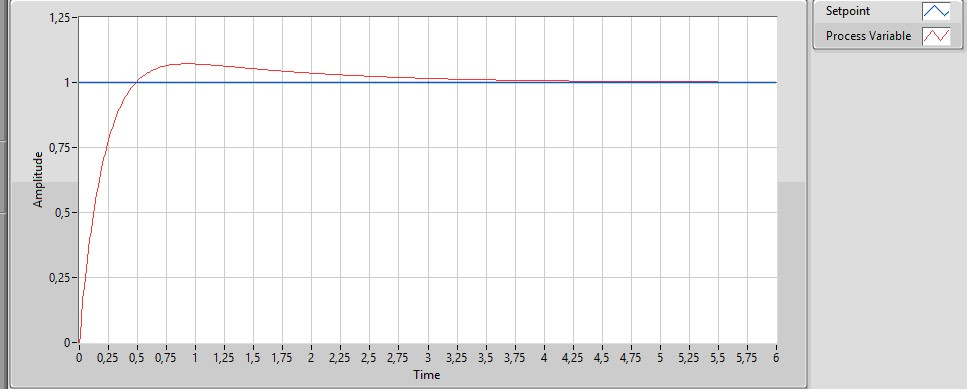
\includegraphics[width=\textwidth,height=5cm,keepaspectratio]{motor_pid_slow_start}
  \caption{Βηματική απόκριση του συστήματος DC κινητήρα όταν αυτός ξεκινάει από την ηρεμία και ελέγχεται με τη χρήση του αυτο-ρυθμιζόμενου PID ελεγκτή}
  \label{fig:motor_pid_slow_start}
\end{figure}

\subsubsection{Αντιμετώπιση Διαταραχών}

Στο Σχήμα \ref{fig:motor_disturbances_slow} φαίνεται πώς το κλειστό σύστημα ελέγχου διαχειρίζεται τις διαταραχές στην είσοδό της συνάρτησης μεταφοράς. Ο ελεγκτής κάνει καλή δουλειά στην αντιμετώπιση του θορύβου που μπορεί να υπεισέρχεται στο σύστημα του DC κινητήρα, κρατώντας την ταχύτητά του κοντά στα επιθυμητά πλαίσια και επαναφέροντάς την γρήγορα όταν οι διαταραχές σταματήσουν.

\begin{figure}[h]
  \centering
  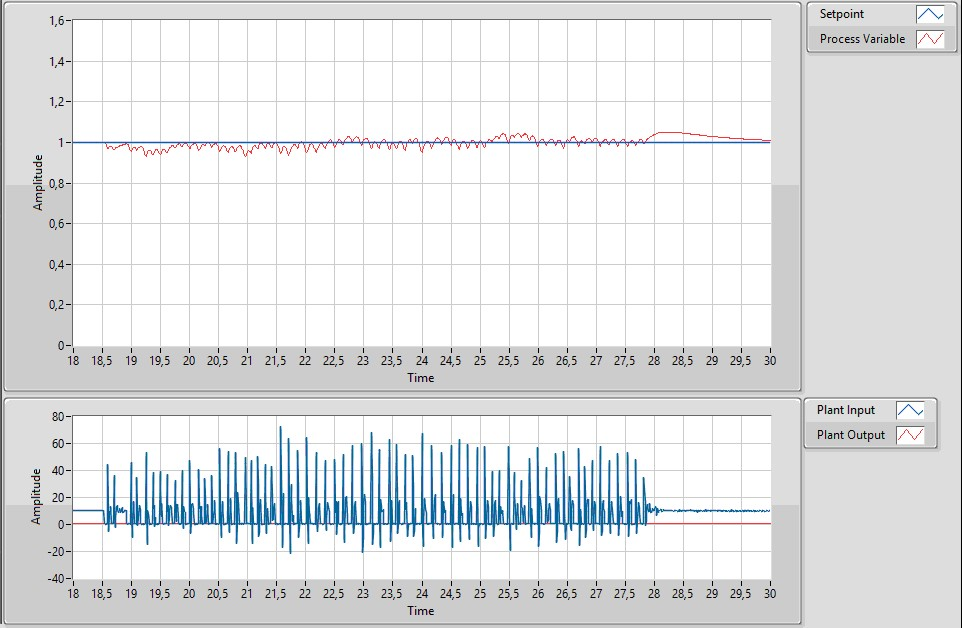
\includegraphics[width=\textwidth,height=5cm,keepaspectratio]{motor_disturbances_slow}
  \caption{Αντιμετώπιση διαταραχών του αυτο-ρυθμιζόμενου PID ελεγκτή του οποίου τα κέρδη έχουν υπολογιστεί με τους τύπους Ziegler-Nichols}
  \label{fig:motor_disturbances_slow}
\end{figure}

\subsection{Αποτελέσματα}

Σε αυτή την ενότητα χρησιμοποιώντας τον αυτο-ρυθμιζόμενο PID ελεγκτή επιχειρήσαμε να ελέγξουμε την ταχύτητα ενός ηλεκτρικού κινητήρα σταθερού ρεύματος.

Αρχικά διαπιστώσαμε ότι χωρίς έλεγχο ο κινητήρας έχει πολύ χαμηλή απόδοση, με τελική γωνιακή ταχύτητα ίση με το ένα δέκατο της επιθυμητής. Στη συνέχεια, προστέθηκε ο αναλογικός όρος του ελεγκτή προκειμένου να δούμε αν αυτός αρκεί για να ελέγξει το σύστημα. Παρόλο που με αυτή την προσθήκη η τελική τιμή της ταχύτητας του ρότορα ήταν πολύ πιο κοντά στην επιθυμητή, παρουσιάζοντας σφάλμα $4.432\%$, οι ταλαντώσεις και η υπερακόντιση που παρουσίασε το σύστημα κατά τη μεταβατική του κατάσταση είναι μη αποδεκτά φαινόμενα, οπότε η χρήση μόνο αναλογικού ελεγκτή απορρίφθηκε σαν λύση ικανοποιητικού ελέγχου.

Φυσικό επακόλουθο ήταν να χρησιμοποιηθεί και ο διαφορικός όρος του ελεγκτή ο οποίος βελτιώνει την ευστάθεια του συστήματος και εξομαλύνει τα αρνητικά φαινόμενα που αναφέρθηκαν. Πράγματι, το διαφορικό κέρδος που υπολόγισε ο αυτο-ρυθμιζόμενος ελεγκτής ήταν ικανό να οδηγήσει σε μια ομαλή πορεία της εξόδου του συστήματος προς το επιθυμητό σημείο. Όμως, δεν είχε καμιά επιρροή στο σφάλμα μόνιμης κατάστασης το οποίο παρέμεινε στην ίδια τιμή.

Σε μια εφαρμογή σαν αυτή, το να πιάσει το σύστημα την είσοδο αναφοράς είναι ίσως το πιο σημαντικό κριτήριο ελέγχου, συνεπώς το σφάλμα μόνιμης κατάστασης έπρεπε να εξαλειφθεί. Οπότε, εισάγαμε στον έλεγχο και τον ολοκληρωτικό όρο του ελεγκτή έτσι ώστε να μηδενιστεί αυτό το σφάλμα. Με τη χρήση και των τριών όρων του, ο αυτο-ρυθμιζόμενος PID ελεγκτής κατάφερε επιτυχώς να καλύψει όλες τις απαιτήσεις ελέγχου. Το σύστημα δεν παρουσιάζει ταλαντώσεις ή υπερακόντιση, έχει μικρό χρόνο ανύψωσης, αντιμετωπίζει ικανοποιητικά τις διαταραχές και έχει μηδενικό σφάλμα μόνιμης κατάστασης.

\section{Σύστημα Inverted Pendulum}

\subsection{Εισαγωγή}

Το σύστημα σε αυτό το παράδειγμα αποτελείται από ένα ανεστραμμένο εκκρεμές τοποθετημένο σε ένα μηχανοκίνητο καροτσάκι. Το σύστημα ανεστραμμένου εκκρεμούς συνήθως συναντάται σε πολλά βιβλία των συστημάτων αυτομάτου ελέγχου καθώς και στην ερευνητική βιβλιογραφία. Η δημοτικότητά του απορρέει εν μέρει από το γεγονός ότι είναι ασταθές χωρίς έλεγχο, δηλαδή το εκκρεμές απλά θα πέσει αν το καλάθι δεν μετακινηθεί για να το ισορροπήσει. Επιπλέον, η δυναμική του συστήματος είναι μη γραμμική. Ο στόχος του συστήματος ελέγχου είναι να ισορροπήσει το ανεστραμμένο εκκρεμές εφαρμόζοντας μια δύναμη στο καλάθι με το εκκρεμές. Ένα παράδειγμα πραγματικού κόσμου που σχετίζεται άμεσα με αυτό το σύστημα ανεστραμμένου εκκρεμούς είναι ο έλεγχος θέσης ενός πυραύλου εκτόξευσης κατά την απογείωση.

Σε αυτή την περίπτωση, θα εξετάσουμε ένα δισδιάστατο πρόβλημα όπου το εκκρεμές είναι περιορισμένο να μετακινείται στο κατακόρυφο επίπεδο που φαίνεται στο παρακάτω σχήμα. Υπό κανονικές συνθήκες, το σύστημα του ανεστραμμένου εκκρεμούς αποτελεί ένα σύστημα μίας εισόδου, δύο εξόδων. Όμως ο PID ελεγκτής μπορεί να ελέγξει ελέγξει συστήματα μίας εισόδου, μίας εξόδου (\emph{Single Input - Single Output} ή \emph{SISO}). Συνεπώς, για το σύστημα αυτό, η είσοδος ελέγχου είναι η δύναμη που κινεί το καλάθι με οριζόντιο τρόπο και η έξοδός του είναι η γωνιακή θέση του εκκρεμούς.

\begin{figure}[h]
  \centering
  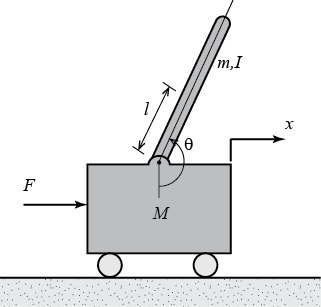
\includegraphics[width=\textwidth,height=5cm,keepaspectratio]{pendulum}
  \caption{Μοντέλο του συστήματος Ανεστραμμένου Εκκρεμούς}
  \label{fig:pendulum}
\end{figure}

\subsection{Μαθηματικό Μοντέλο}

Στο παρακάτω σχήμα φαίνεται το διάγραμμα ελευθέρου σώματος για το σύστημα ανεστραμμένου εκκρεμούς.

\begin{figure}[h]
  \centering
  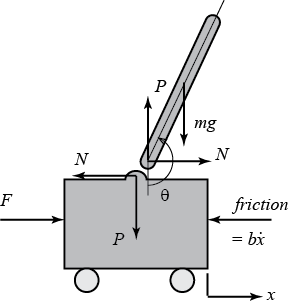
\includegraphics[width=\textwidth,height=5cm,keepaspectratio]{pendulum2}
  \caption{Διάγραμμα ελευθέρου σώματος για το σύστημα ανεστραμμένου εκκρεμούς}
  \label{fig:pendulum2}
\end{figure}

Συγκεντρώνοντας τις δυνάμεις στο διάγραμμα ελεύθερου σώματος του καροτσιού στην οριζόντια κατεύθυνση, έχουμε την ακόλουθη εξίσωση κίνησης
\begin{equation}
M\ddot{x} + b\dot{x} + N = F
\end{equation}
Συγκεντρώνοντας τις δυνάμεις στο διάγραμμα ελεύθερου σώματος του εκκρεμούς στην οριζόντια κατεύθυνση, λαμβάνουμε την ακόλουθη έκφραση για τη δύναμη αντίδρασης $N$
\begin{equation}
N = m\ddot{x} + ml\ddot{\theta}\cos{\theta} - ml\dot{\theta}^2\sin{\theta}
\end{equation}
Αν αντικαταστήσουμε αυτή την εξίσωση στην πρώτη εξίσωση, παίρνουμε μια από τις δύο εξισώσεις που ισχύουν για αυτό το σύστημα
\begin{equation}
(M+m)\ddot{x} + b\dot{x} + ml\ddot{\theta}\cos{\theta}-ml\dot{\theta}^2\sin{\theta} = F
\end{equation}
Για να πάρουμε τη δεύτερη εξίσωση κίνησης για αυτό το σύστημα, αθροίζουμε τις δυνάμεις κάθετες στο εκκρεμές. Η εξίσωση που προκύπτει είναι η ακόλουθη
\begin{equation}
P\sin{\theta}+N\cos{\theta}-mg\sin{\theta}=ml\ddot{\theta}+m\ddot{x}\cos{\theta}
\end{equation}
Για να απαλλαγούμε από τους όρους της παραπάνω εξίσωσης, αθροίζουμε τις ροπές του εκκρεμούς για να πάρουμε την ακόλουθη εξίσωση
\begin{equation}
-Pl\sin{\theta}-Nl\cos{\theta}=I\ddot{\theta}
\end{equation}
Συνδυάζοντας αυτές τις δύο τελευταίες εκφράσεις, παίρνουμε τη δεύτερη εξίσωση κίνησης
\begin{equation}
\left(I+ml^2\right)\ddot{\theta}+mgl\sin{\theta}=-ml\ddot{x}\cos{\theta}
\end{equation}
Δεδομένου ότι οι τεχνικές ανάλυσης και σχεδιασμού ελέγχου που θα χρησιμοποιήσουμε σε αυτό το παράδειγμα ισχύουν μόνο για γραμμικά συστήματα, αυτό το σύνολο εξισώσεων πρέπει να γραμμικοποιηθεί. Συγκεκριμένα, θα γραμμικοποιήσουμε τις εξισώσεις σχετικά με την κατακόρυφη ανοδική θέση $\theta=\pi$, και θα υποθέσουμε ότι το σύστημα παραμένει μέσα σε μια μικρή γειτονιά αυτής της ισορροπίας. Αυτή η παραδοχή θα πρέπει να είναι λογικά έγκυρη αφού υπό τον έλεγχο θέλουμε το εκκρεμές να μην αποκλίνει πολύ από την κάθετα προς τα άνω θέση. Έστω ότι $\phi$ είναι η απόκλιση της θέσης του εκκρεμούς από την ισορροπία, δηλαδή, $\theta=\pi+\phi$. Συνεπώς, υποθέτωντας μια μικρή απόκλιση ($\phi$) από την ισορροπία, μπορούμε να χρησιμοποιήσουμε τις παρακάτω προσεγγίσεις μικρών γωνιών των μη γραμμικών συναρτήσεων στις εξισώσεις του συστήματός μας
\begin{equation}
\cos\theta=\cos(\pi+\phi)\approx -1
\end{equation}
\begin{equation}
\sin\theta=\sin(\pi+\phi)\approx -\phi
\end{equation}
\begin{equation}
\dot{\theta}^2=\dot{\phi}^2\approx 0
\end{equation}
Αφού αντικαταστήσουμε τις παραπάνω προσεγγίσεις στις μη γραμμικές εξισώσεις μας, φτάνουμε στις δύο γραμμικές εξισώσεις κίνησης. Το σύμβολο της εισόδου $F$ αντικαταστάθηκε από το σύμβολο $u$.
\begin{equation}
\left(I+ml^2\right)\ddot{\phi}-mgl\phi=ml\ddot{x}
\end{equation}
\begin{equation}
\left(M+m\right)\ddot{x}+b\dot{x}-ml\ddot{\phi}=u
\end{equation}
Για να λάβουμε τις συναρτήσεις μεταφοράς των εξισώσεων του γραμμικού συστήματος, πρέπει πρώτα να πάρουμε το μετασχηματισμό Laplace των εξισώσεων αυτών, υποθέτοντας μηδενικές αρχικές συνθήκες. Οι μετασχηματισμοί Laplace που προκύπτουν παρουσιάζονται παρακάτω.
\begin{equation}
\left(I+ml^2\right)\Phi(s)s^2-mgl\Phi(s)=mlX(s)s^2
\end{equation}
\begin{equation}
\left(M+m\right)X(s)s^2+bX(s)s-ml\Phi(s)s^2=U(s)
\label{eq:inverted_pendulum_5_28}
\end{equation}
Όπως είναι γνωστό, μια συνάρτηση μεταφοράς αντιπροσωπεύει τη σχέση μεταξύ μιας μόνο εισόδου και μιας μόνο εξόδου κάθε φορά. Για να βρούμε τη συνάρτηση μεταφοράς για την έξοδο $\Phi(s)$ και της εισόδου $U(s)$ πρέπει να εξαλείψουμε το $X(s)$ από τις παραπάνω εξισώσεις. Λύνοντας την πρώτη εξίσωση ως προς το $X(s)$ έχουμε
\begin{equation}
X(s) = \left[\frac{I+ml^2}{ml}-\frac{g}{s^2}\right]\Phi(s)
\end{equation}
Αντικαθιστώντας αυτή την εξίσωση στην εξίσωση \ref{eq:inverted_pendulum_5_28} έχουμε
\begin{equation}
\left(M+m\right)\left[\frac{I+ml^2}{ml}\frac{g}{s^2}\right]\Phi(s)s^2+b\left[\frac{I+ml^2}{ml}\frac{g}{s^2}\right]\Phi(s)s-ml\Phi(s)s^2=U(s)
\end{equation}
Αναδιατάσσοντας την εξίσωση αυτή παίρνουμε τη συνάρτηση μεταφοράς
\begin{equation}
\frac{\Phi(s)}{U(s)} = \frac{\frac{ml}{q}s}{s^3+\frac{b(I+ml^2)}{q}s^2-\frac{(M+m)mgl}{q}s-\frac{bmgl}{q}} \left[\frac{rad}{N}\right]
\end{equation}
όπου,
\begin{equation}
q = \left(M+m\right)\left(I+ml^2\right)-\left(ml\right)^2
\end{equation}

\subsection{Πείραμα}

Υποθέτουμε ότι για αυτό το παράδειγμα οι παράμετροι του συστήματος είναι ως εξής
\begin{flushleft}
\begin{tabular}{lll}
$\mathbf{M}$ & μάζα του καροτσιού & $0.5\ kg$ \\  
$\mathbf{m}$ & μάζα του εκκρεμούς & $0.2\ kg$ \\ 
$\mathbf{b}$ & σταθερά τριβής για το καρότσι & $0.1 \frac{N}{m/s}$ \\ 
$\mathbf{l}$ & απόσταση του κέντρου μάζας του εκκρεμούς & $0.3\ m$ \\ 
$\mathbf{I}$ & ροπή αδράνειας του εκκρεμούς & $0.006\ kgm^2$ \\ 
\end{tabular}
\end{flushleft}
 
Το πείραμα αυτή τη φορά είναι λίγο διαφορετικό από τα προηγούμενα. Όπως αναφέρθηκε, το συγκεκριμένο σύστημα κανονικά έχει μία είσοδο και δύο εξόδους. Για να προσαρμοστεί όμως στον PID έλεγχο αγνοήσαμε τη μία έξοδο που αποτελούσε τη θέση του καροτσιού. Ως αποτέλεσμα και η πειραματική διαδικασία θα πρέπει να υπόκειται σε κάποιους περιορισμούς.

Πιο συγκεκριμένα, θα θεωρήσουμε ότι το εκκρεμές είναι ήδη ακίνητο στην κατακόρυφη θέση $\theta = \pi$. Αυτό σημαίνει ότι η επιθυμητή τιμή είναι setpoint $=0$. Για τον έλεγχο του συστήματος θα σπρώχνουμε στιγμιαία το καρότσι, δηλαδή θα εισάγουμε μια κρουστική με τη μορφή διαταραχής στο σύστημα. Στόχος του ελέγχου θα είναι ο αυτο-ρυθμιζόμενος PID ελεγκτής να υπολογίσει τα κέρδη έτσι ώστε το εκκρεμές να επανέρχεται στην κατακόρυφη θέση χωρίς να απομακρύνεται πολύ από αυτή. 

Επίσης, προκειμένου να υπολογίσει ο αλγόριθμος το κατάλληλο αναλογικό κέρδος το σύστημα θα πρέπει να υποστεί τη διαδικασία των ταλαντώσεων λόγω του relay στοιχείου. Επειδή το σύστημα είναι από μόνο του ασταθές, οι ταλαντώσεις αυτές δε θα έχουν σταθερό πλάτος οδηγώντας μετά από λίγο το σύστημα στην αστάθεια (βλέπε Σχήμα \ref{fig:pendulum_relay}). Προκειμένου λοιπόν να βρει ο αλγόριθμος κάποιες τιμές για τα κέρδη το πείραμα θα διακόπτεται πριν η απόκριση του συστήματος τείνει στο άπειρο. 

\begin{figure}[h]
  \centering
  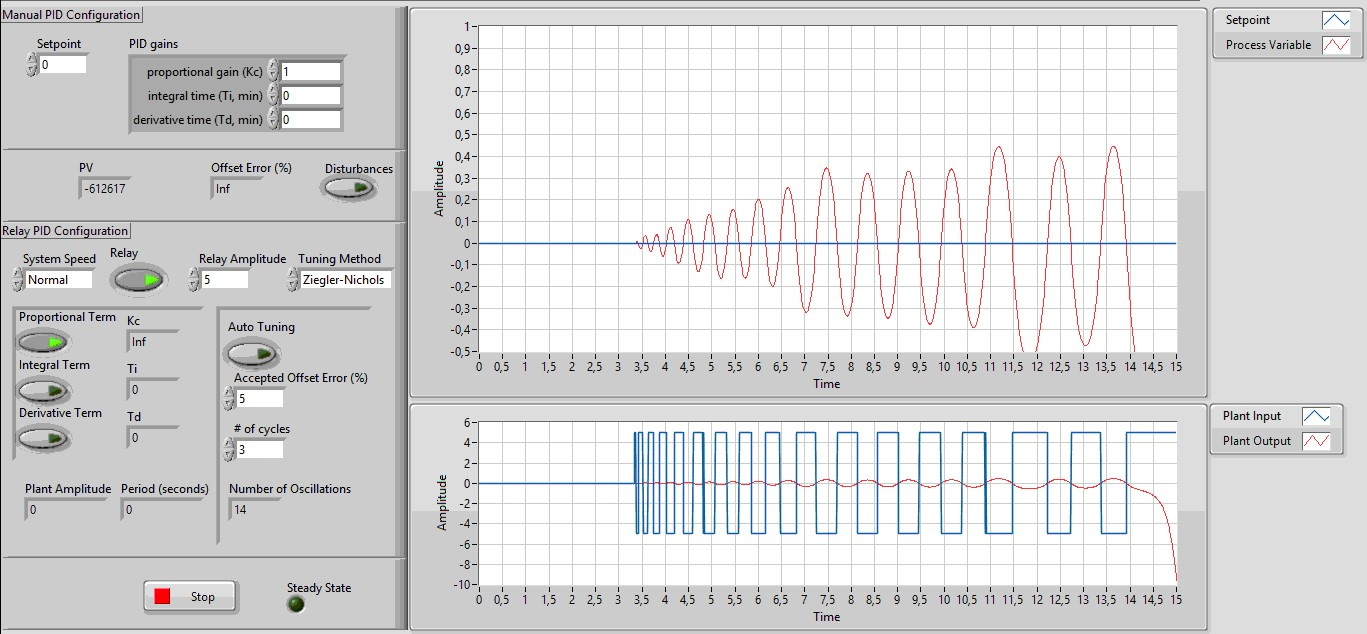
\includegraphics[width=\textwidth,height=5cm,keepaspectratio]{pendulum_relay}
  \caption{Απόκριση του συστήματος κατά τη διάρκεια του relay πειράματος}
  \label{fig:pendulum_relay}
\end{figure}

\subsubsection{Απόκριση Χωρίς Έλεγχο}

\begin{figure}[h]
  \centering
  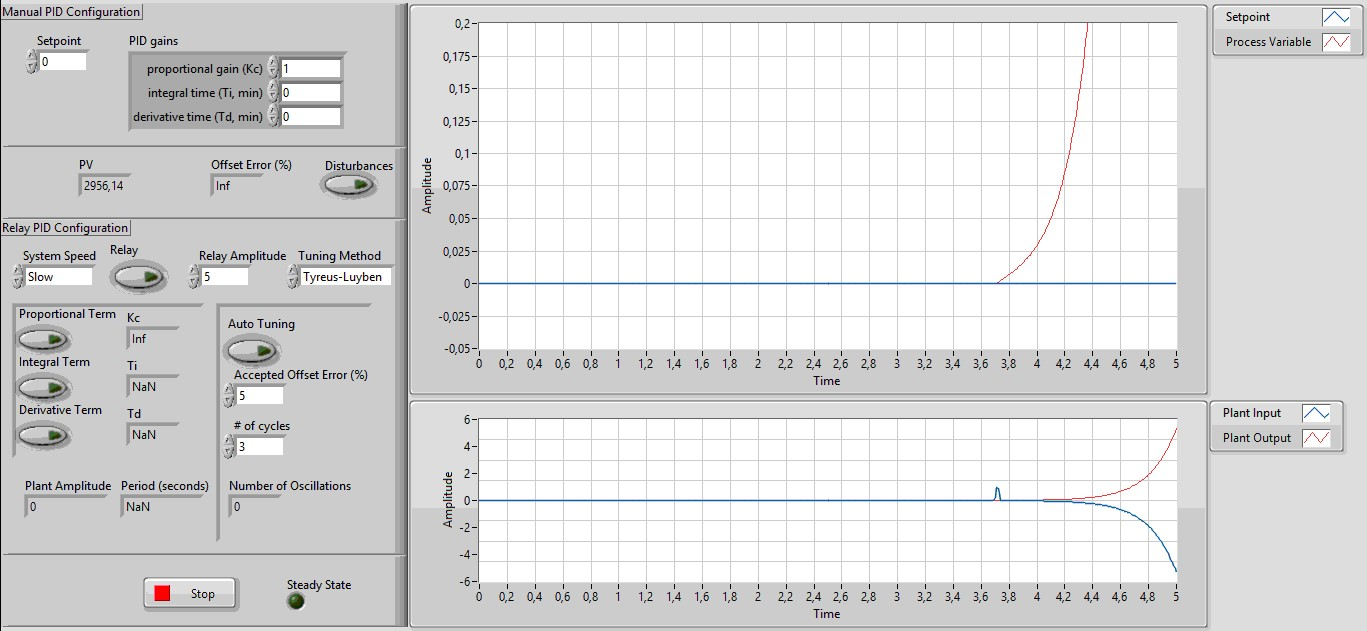
\includegraphics[width=\textwidth,height=5cm,keepaspectratio]{pendulum_no_control}
  \caption{Απόκριση του συστήματος Ανεστραμμένου Εκκρεμούς χωρίς έλεγχο}
  \label{fig:pendulum_no_control}
\end{figure}

Από το παραπάνω σχήμα γίνεται εύκολα αντιληπτό ότι το σύστημα όταν λειτουργεί χωρίς έλεγχο είναι ασταθές. Μια μικρή διαταραχή έχει ως αποτέλεσμα η γωνία απόκλισης του εκκρεμούς να τείνει στο άπειρο.

\subsubsection{Αναλογικός Έλεγχος}

Τώρα θα γίνει προσπάθεια να ελεγχθεί το σύστημα χρησιμοποιώντας μόνο τον αναλογικό όρο. Η προσπάθεια αυτή αναπαρίσταται στο Σχήμα \ref{fig:pendulum_proportional}.

\begin{figure}[h]
  \centering
  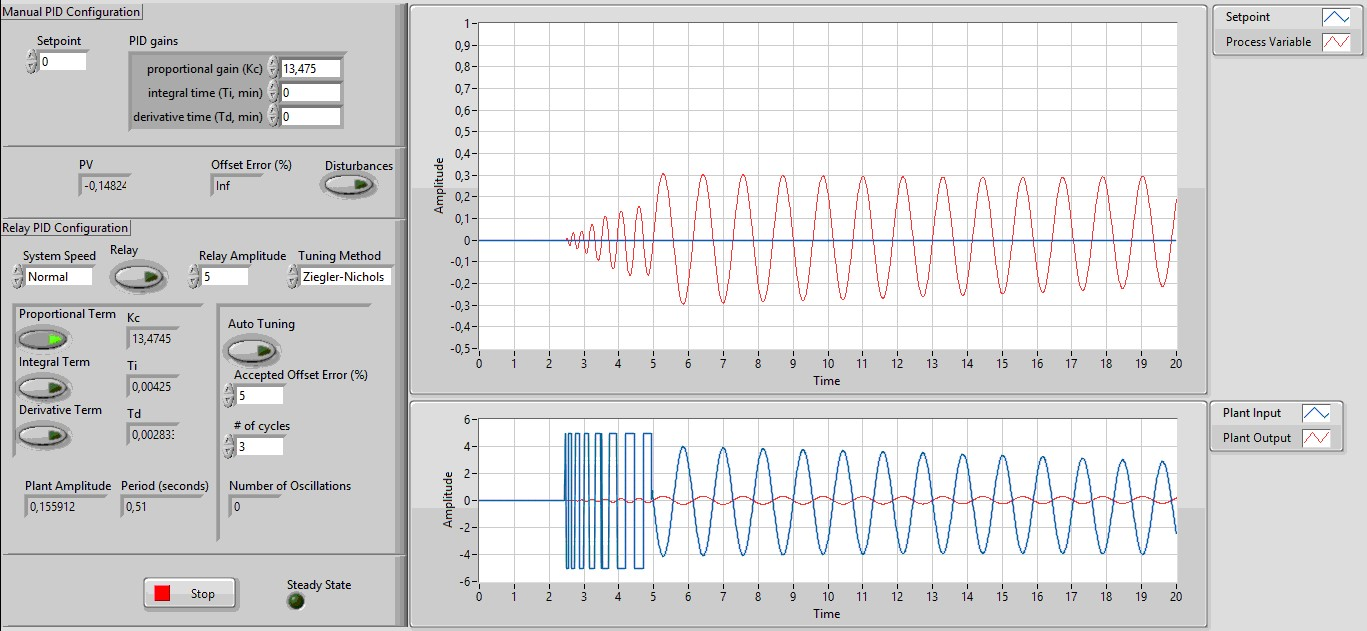
\includegraphics[width=\textwidth,height=5cm,keepaspectratio]{pendulum_proportional}
  \caption{Απόκριση του συστήματος ανεστραμμένου εκκρεμούς με εφαρμογή αναλογικού ελέγχου}
  \label{fig:pendulum_proportional}
\end{figure}
Μετά το πέμπτο δευτερόλεπτο διακόπτουμε το πείραμα relay. Το αναλογικό κέρδος που έχει υπολογιστεί είναι $K_c=13.475$. Αυτό το κέρδος δεν είναι ικανό να επαναφέρει το εκκρεμές στην αρχική του θέση, αλλά ούτε το ωθεί στην αστάθεια αφού εκτελεί αμείωτες ταλαντώσεις. 

\subsubsection{Αναλογικός - Διαφορικός Έλεγχος}

\begin{figure}[h]
  \centering
  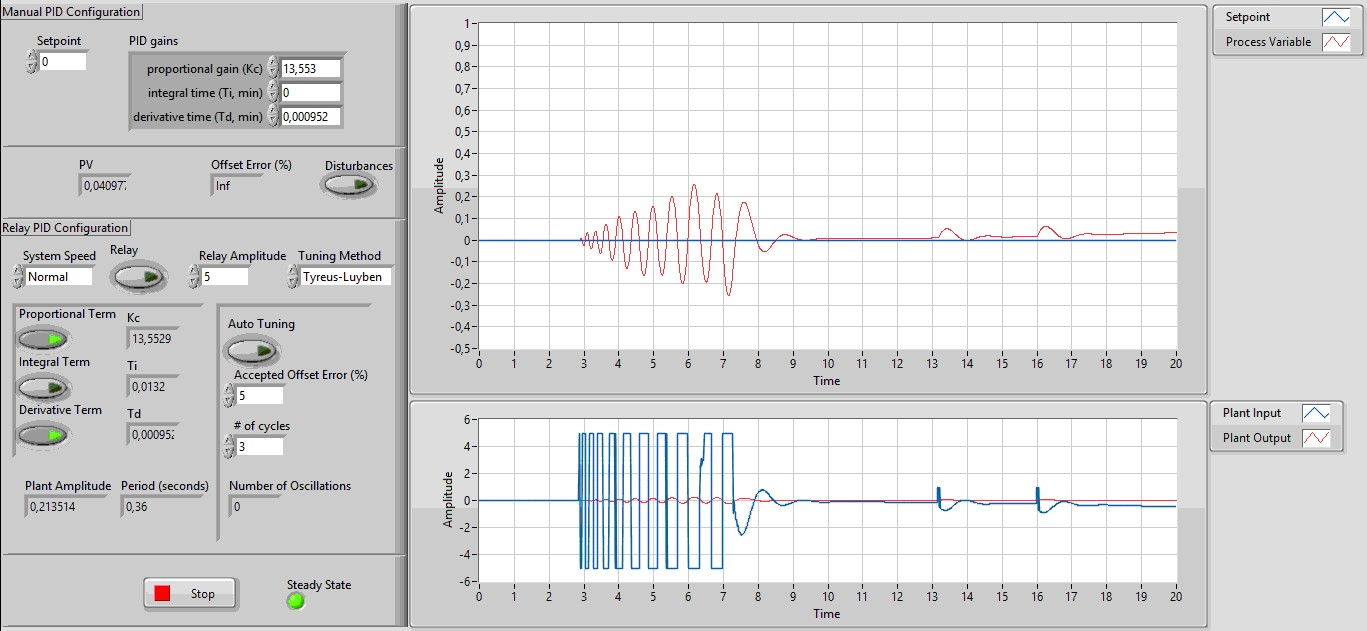
\includegraphics[width=\textwidth,height=5cm,keepaspectratio]{pendulum_pd}
  \caption{Απόκριση του συστήματος ανεστραμμένου εκκρεμούς με εφαρμογή αναλογικού - διαφορικού ελέγχου}
  \label{fig:pendulum_pd}
\end{figure}

Στη συνέχεια προστίθεται και ο διαφορικός όρος προκειμένου να βελτιωθεί η ευστάθεια του συστήματος και να μετριαστούν οι ταλαντώσεις. Επίσης, οι τύποι για τον υπολογισμό των κερδών για τη συνέχεια του πειράματος θα είναι αυτή που βασίζονται στη μέθοδο Tyreus-Luyben επειδή προσφέρουν μια λιγότερο ``επιθετική" προσέγγιση στον έλεγχο του συστήματος. Η απόκριση του συστήματος φαίνεται στο παραπάνω σχήμα.

Η βελτίωση στην απόκριση του συστήματος είναι εμφανής. Οι τιμές των όρων του ελεγκτή που υπολογίστηκαν από το πείραμα relay ($K_c = 13.553,\ T_d = 0,000952$) είναι ικανές να φέρουν το σύστημα πολύ κοντά στην αρχική του θέση. Επίσης οι κρουστικές διαταραχές δεν το απομακρύνουν πολύ από τη θέση ισορροπίας του. Όμως με μια προσεκτική ματιά παρατηρούμε ότι η γωνία του εκκρεμούς ολοένα και αυξάνεται, αργά αλλά σταθερά. Συνεπώς ούτε τώρα το σύστημα είναι απολύτως ευσταθές, απλά αργεί πολύ περισσότερο να οδηγηθεί στην αστάθεια.

\subsubsection{Αναλογικός - Ολοκληρωτικός - Διαφορικός Έλεγχος}

\begin{figure}[h]
  \centering
  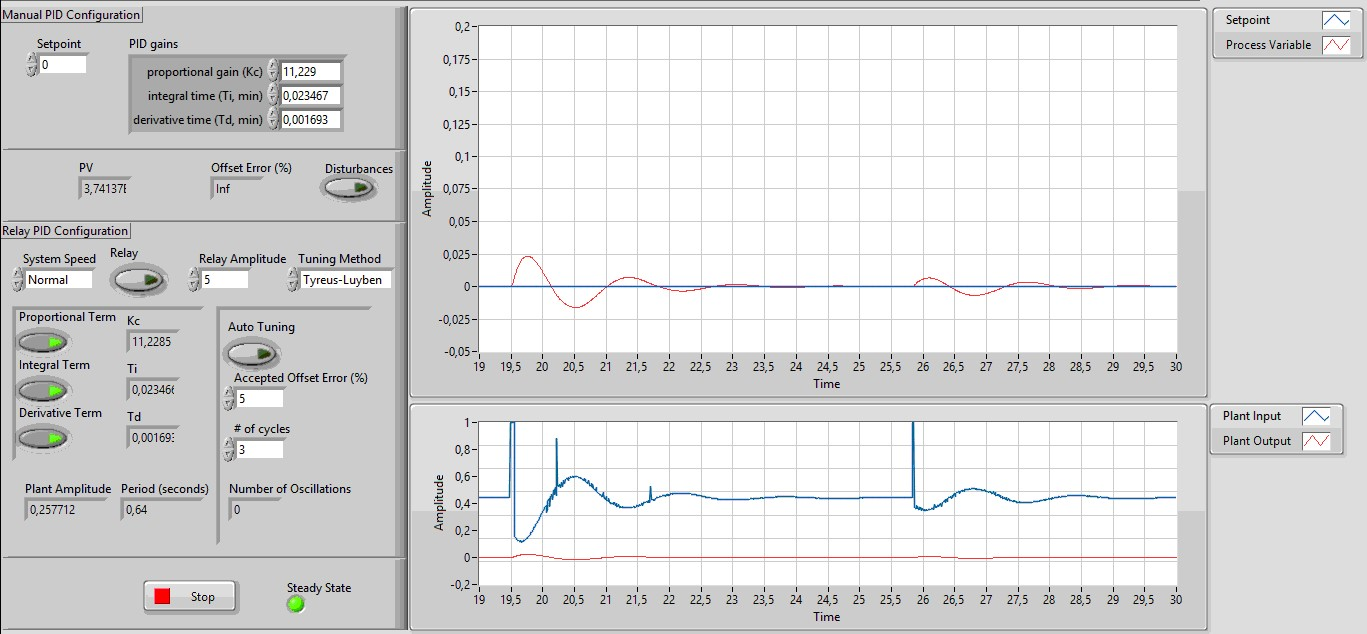
\includegraphics[width=\textwidth,height=5cm,keepaspectratio]{pendulum_pid}
  \caption{Απόκριση του συστήματος ανεστραμμένου εκκρεμούς με εφαρμογή αναλογικού - ολοκληρωτικού - διαφορικού ελέγχου}
  \label{fig:pendulum_pid}
\end{figure}

Στο παραπάνω σχήμα φαίνεται η απόκριση του συστήματος όταν εφαρμόζεται PID έλεγχος. Πλέον ο ελεγκτής είναι ικανός να επαναφέρει το σύστημα στην αρχική του θέση. Επίσης, όταν εφαρμόζονται κρουστικές διαταραχές ο έλεγχος δεν αφήνει το εκκρεμές να απομακρυνθεί πολύ από τη θέση ισορροπίας και η επαναφορά του σε αυτή γίνεται σε μικρό χρονικό διάστημα. 

\subsubsection{Αποτελέσματα}

Σε αυτή την ενότητα ο αυτο-ρυθμιζόμενος PID ελεγκτής επιχείρησε να ελέγξει ένα αρκετά απαιτητικό σύστημα. Το ανεστραμμένο εκκρεμές είναι ένα εν γένει μη γραμμικό, ασταθές σύστημα, μίας εισόδου -- δύο εξόδων. Αυτό οδήγησε σε αρκετούς συμβιβασμούς στον έλεγχο.

Αρχικά το σύστημα έπρεπε να γραμμικοποιηθεί γύρω από την κατακόρυφη θέση ισορροπίας του $\theta = \pi$. Ως αποτέλεσμα αυτού, η συνάρτηση μεταφοράς του ισχύει μόνο για μικρές αποκλίσεις της γωνίας του εκκρεμούς από την αρχική του θέση. Επίσης, επειδή ο PID έλεγχος χρησιμοποιείται για έλεγχο συστημάτων μίας εισόδου -- μίας εξόδου, αγνοήσαμε εντελώς τη θέση του καροτσιού και λάβαμε υπόψιν μας μόνο τη γωνία του εκκρεμούς. Τέλος, λόγω της εκ φύσεως αστάθειας του συστήματος, το πείραμα relay μέσω του οποίου ο αλγόριθμος εκτιμά τις τιμές των όρων του ελεγκτή δεν οδηγούσε σε σταθερές αμείωτες ταλαντώσεις οπότε έπρεπε να διακόπτεται πριν το σύστημα οδηγηθεί στην αστάθεια. 

Όμως, παρόλες τις δυσκολίες ελέγχου, ο αυτο--ρυθμιζόμενος PID ελεγκτής πρόσφερε μια ικανοποιητική λύση για το συγκεκριμένο πρόβλημα. Παρότι τα κέρδη υπολογίζονται χρησιμοποιώντας ταλαντώσεις μη σταθερού πλάτους, οι τιμές που τους αποδίδονται κρίνονται επαρκής για τις απαιτήσεις ελέγχου ενός τέτοιου συστήματος. Με τη χρήση και των τριών όρων του δεν αφήνει το εκκρεμές να αποκλίνει πολύ από τη θέση ισορροπίας του όταν υπεισέρχονται διαταραχές στο σύστημα. Επίσης το επαναφέρει στην αρχική του θέση σε λιγότερο από πέντε δευτερόλεπτα και εμφανίζει μηδενικό σφάλμα μόνιμης κατάστασης. Με λίγα λόγια το σύστημα πλέον είναι ευσταθές, με ανοχή σε στιγμιαίες διαταραχές και συνεπώς η αυτόματη ρύθμιση του PID ελεγκτή κρίνεται επιτυχής.

\section{Σύστημα Aircraft Pitch}

\begin{figure}[h]
  \centering
  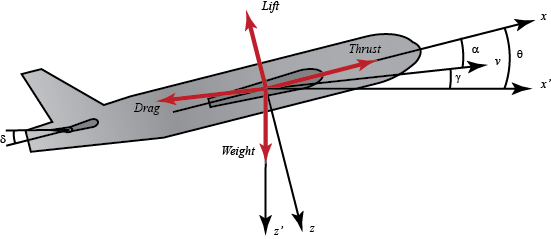
\includegraphics[width=\textwidth,height=5cm,keepaspectratio]{flightdynamics}
  \caption{Μοντέλο του συστήματος Αεροσκάφους}
  \label{fig:flightdynamics}
\end{figure}

\subsection{Εισαγωγή}

Σε αυτή την ενότητα θα γίνει προσπάθεια να σχεδιασθεί ένας αυτόματος πιλότος που θα ελέγχει το βήμα ενός αεροσκάφους (\emph{aircraft pitch}).

\subsection{Μαθηματικό Μοντέλο}
Οι βασικοί άξονες και δυνάμεις των συντεταγμένων που δρουν σε ένα αεροσκάφος παρουσιάζονται στο Σχήμα \ref{fig:flightdynamics}. Οι εξισώσεις που διέπουν την κίνηση ενός αεροσκάφους είναι ένα πολύ περίπλοκο σύνολο έξι μη γραμμικών συζευγμένων διαφορικών εξισώσεων. Ωστόσο, με ορισμένες υποθέσεις, μπορούν να αποσυνδεθούν και να γραμμικοποιηθούν σε διαμήκεις και πλευρικές εξισώσεις. Σύμφωνα με αυτές τις υποθέσεις, οι διαμήκεις εξισώσεις κίνησης του αεροσκάφους μπορούν να γραφτούν ως εξής
\begin{equation}
\dot{\alpha}=\mu\Omega\sigma\left[-\left(C_L+C_D\right)\alpha+\frac{1}{\mu-C_L}q-\left(C_W\sin\gamma\right)\theta+C_L\right]
\end{equation}
\begin{equation}
\dot{q}=\frac{\mu\Omega}{2i_{yy}}\left[\left[C_M-\eta\left(C_L+C_D\right)\right]\alpha+\left[C_M+\sigma C_M\left(1-\mu C_L\right)\right]q+\left(\eta C_W\sin\gamma\right)\delta\right]
\end{equation}
\begin{equation}
\dot{\theta}=\Omega q
\end{equation}
Το πώς προκύπτουν αυτές οι εξισώσεις μπορεί να βρεθεί σε οποιοδήποτε διδακτικό βιβλίο σχετικά με αεροσκάφη. Για το σύστημα αυτό, η είσοδος θα είναι η γωνία κλίσης $\delta$ και η έξοδος θα είναι η γωνία βήματος $\theta$ του αεροσκάφους.

Πριν από την εύρεση της συνάρτησης μεταφοράς, ας συνδέσουμε μερικές αριθμητικές τιμές για να απλοποιήσουμε τις παραπάνω εξισώσεις μοντελοποίησης:
\begin{equation}
\dot{\alpha} = -0.313\alpha + 56.7q + 0.232\delta
\end{equation}
\begin{equation}
\dot{q} = -0.0139\alpha - 0.426q + 0.0203\delta
\end{equation}
\begin{equation}
\dot{\theta} = 56.7q
\end{equation}
Αυτές οι τιμές λαμβάνονται από τα δεδομένα ενός εμπορικού αεροσκάφους της Boeing.

Για να βρούμε τη συνάρτηση μεταφοράς του παραπάνω συστήματος, πρέπει να πάρουμε το μετασχηματισμό Laplace των παραπάνω εξισώσεων μοντελοποίησης. Για την εύρεση της συνάρτησης μεταφοράς θεωρούμε μηδενικές αρχικές συνθήκες. Ο μετασχηματισμός Laplace των παραπάνω εξισώσεων παρουσιάζεται παρακάτω
\begin{equation}
sA(s)=-0.313A(s)+56.7Q(s)+0.232\Delta(s)
\end{equation}
\begin{equation}
sQ(s)=-0.0139A(s)-0.426Q(s)+0.0203\Delta(s)
\end{equation}
\begin{equation}
s\Theta(s) = 56.7Q(s)
\end{equation}
Μετά από μερικές απλές αλγεβρικές πράξεις καταλήγουμε στην ακόλουθη συνάρτηση μεταφοράς
\begin{equation}
P(s) = \frac{\Theta(s)}{\Delta(s)} = \frac{1.151s+0.1774}{s^3+0.739s^2+0.921s}
\label{eq:aircraft_tf}
\end{equation}

\subsection{Πείραμα}

Σε αυτό το παράδειγμα θέλουμε να δούμε αν ο αυτο-ρυθμιζόμενος PID ελεγκτής είναι σε θέση να ελέγξει ικανοποιητικά τη γωνία κλίσης του αεροσκάφους. Συγκεκριμένα, θέλουμε για βηματική είσοδο αναφοράς να μην παρουσιάζει μεγάλη υπερακόντιση, να μην έχει υπερβολικά μεγάλο χρόνο ανύψωσης και να παρουσιάζει πολύ μικρό σφάλμα μόνιμης κατάστασης. Στο πείραμα η είσοδος θα έχει τιμή $\delta=0.2$ rad (περίπου 11 μοίρες).

\subsubsection{Απόκριση Χωρίς Έλεγχο}

\begin{figure}[h]
  \centering
  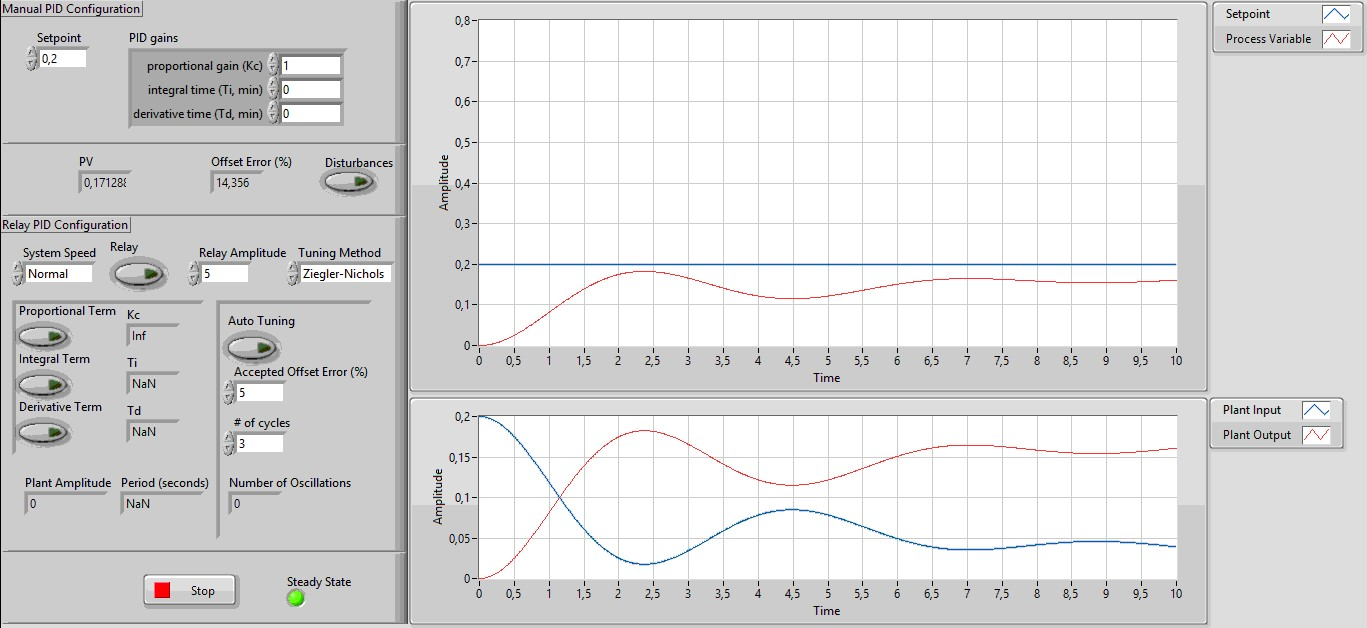
\includegraphics[width=\textwidth,height=5cm,keepaspectratio]{aircraft_no_control}
  \caption{Απόκριση του αεροσκάφους σε είσοδο $\delta = 0.2$ rad χωρίς τη χρήση ελέγχου}
  \label{fig:aircraft_no_control}
\end{figure}

Όπως φαίνεται και από το παραπάνω σχήμα, το σύστημα όταν δρα χωρίς ελεγκτή δεν είναι ικανό να καλύψει τις απαιτήσεις ελέγχου. Ενώ η απόκριση του δεν παρουσιάζει υπερακόντιση, είναι σχετικά αργή και έχει ποσοστό σφάλματος μόνιμης κατάστασης περίπου $14\%$.

\subsubsection{Αναλογικός Έλεγχος}

\begin{figure}[h]
  \centering
  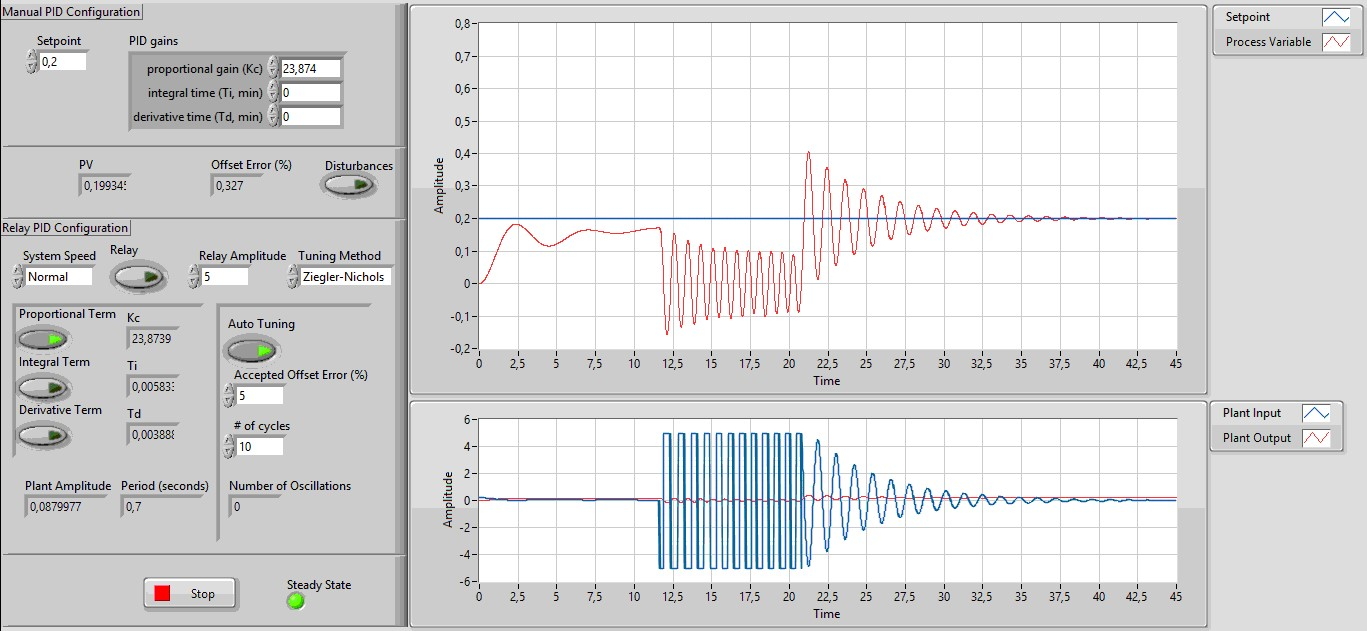
\includegraphics[width=\textwidth,height=5cm,keepaspectratio]{aircraft_p}
  \caption{Απόκριση του αεροσκάφους σε είσοδο $\delta = 0.2$ rad με τη χρήση αναλογικού ελέγχου}
  \label{fig:aircraft_p}
\end{figure}

Στο Σχήμα \ref{fig:aircraft_p} φαίνεται η απόκριση του συστήματος όταν σε αυτό εφαρμόζεται μόνο ο αναλογικός έλεγχος του PID ελεγκτή. Ο PID ελεγκτής έχει ρυθμιστεί στη λειτουργία ``Auto Tuning", συνεπώς μόλις ανιχνεύσει μόνιμο σφάλμα πάνω από $5\%$ για περισσότερο από πέντε δευτερόλεπτα εκτελεί αυτόματα το πείραμα relay. Δέκα ταλαντώσεις μετά, και ενώ το πλάτος τους είναι \emph{περίπου} σταθερό, ο αλγόριθμος διακόπτει το πείραμα και θέτει σε λειτουργία πάλι τον ελεγκτή χρησιμοποιώντας μόνο τον αναλογικό του όρο. Από τη γραφική παράσταση βλέπουμε ότι το μόνιμο σφάλμα είναι μικρότερο από $1\%$ αλλά η απόκριση παρουσιάζει υπερβολική υπερακόντιση και ταλαντώσεις.

\subsubsection{Αναλογικός -- Διαφορικός Έλεγχος}

Αφού το μόνιμο σφάλμα βρίσκεται σε ικανοποιητικά επίπεδα, η χρήση του ολοκληρωτικού όρου κρίνεται περιττή για το συγκεκριμένο σύστημα. Για τη βελτίωση της μεταβατικής κατάστασης εισάγουμε τον διαφορικό όρο. Η προσθήκη αυτή έχει εμφανή αποτελέσματα στην απόκριση του συστήματος όπως φαίνεται και στο παρακάτω σχήμα.

\begin{figure}[h]
  \centering
  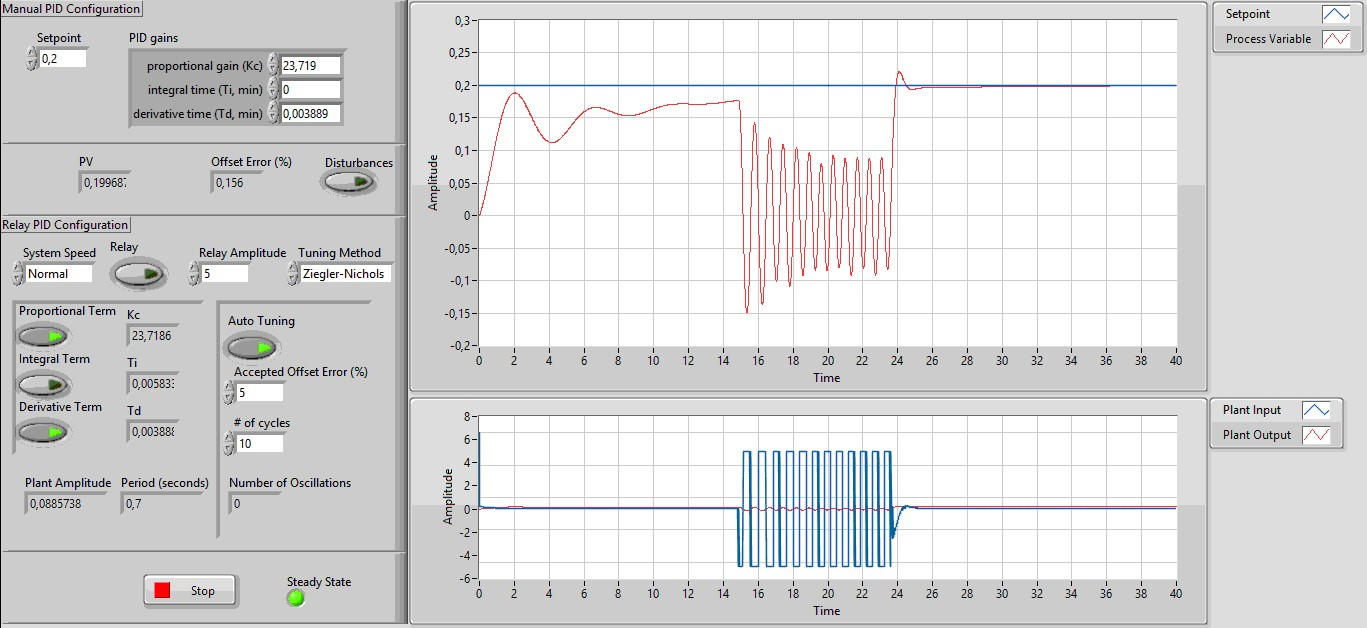
\includegraphics[width=\textwidth,height=5cm,keepaspectratio]{aircraft_pd}
  \caption{Απόκριση του αεροσκάφους σε είσοδο $\delta = 0.2$ rad με τη χρήση αναλογικού -- διαφορικού ελέγχου}
  \label{fig:aircraft_pd}
\end{figure}

\subsubsection{Άλλες Αποκρίσεις}

Εδώ φαίνονται οι αποκρίσεις του συστήματος για διαφορετικές ρυθμίσεις του προγράμματος. Συγκεκριμένα, στο Σχήμα \ref{fig:aircraft_pd_slow} φαίνεται η απόκριση του συστήματος όταν τα κέρδη έχουν υπολογιστεί με τους τύπους Ziegler -- Nichols και η επιθυμητή ταχύτητα έχει ρυθμιστεί στο ``Slow", ενώ στο Σχήμα \ref{fig:aircraft_pd_TL} φαίνεται η απόκριση όταν τα κέρδη έχουν υπολογιστεί με τους τύπους Tyreus -- Luyben.

Στην πρώτη περίπτωση το σύστημα δεν παρουσιάζει καθόλου υπερακόντιση κάτι που είναι θετικό αλλά όχι αναγκαίο. Στη δεύτερη περίπτωση η υπερακόντιση του συστήματος είναι μεγαλύτερη από αυτή στις προηγούμενες περιπτώσεις χωρίς ιδιαίτερη διαφορά στο χρόνο ανύψωσης.

\begin{figure}[h]
  \centering
  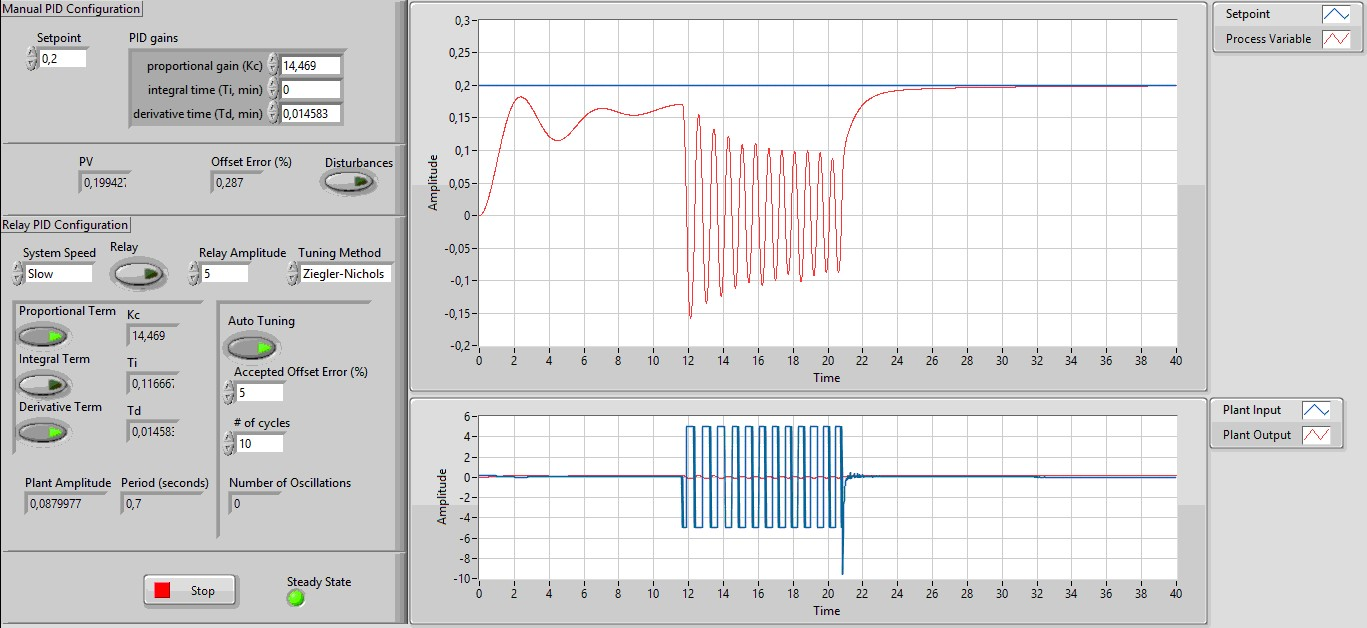
\includegraphics[width=\textwidth,height=5cm,keepaspectratio]{aircraft_pd_slow}
  \caption{Απόκριση του αεροσκάφους σε είσοδο $\delta = 0.2$ rad με τη χρήση αναλογικού -- διαφορικού ελέγχου και επιθυμητή ταχύτητα απόκρισης ``Slow"}
  \label{fig:aircraft_pd_slow}
\end{figure}

\begin{figure}[h]
  \centering
  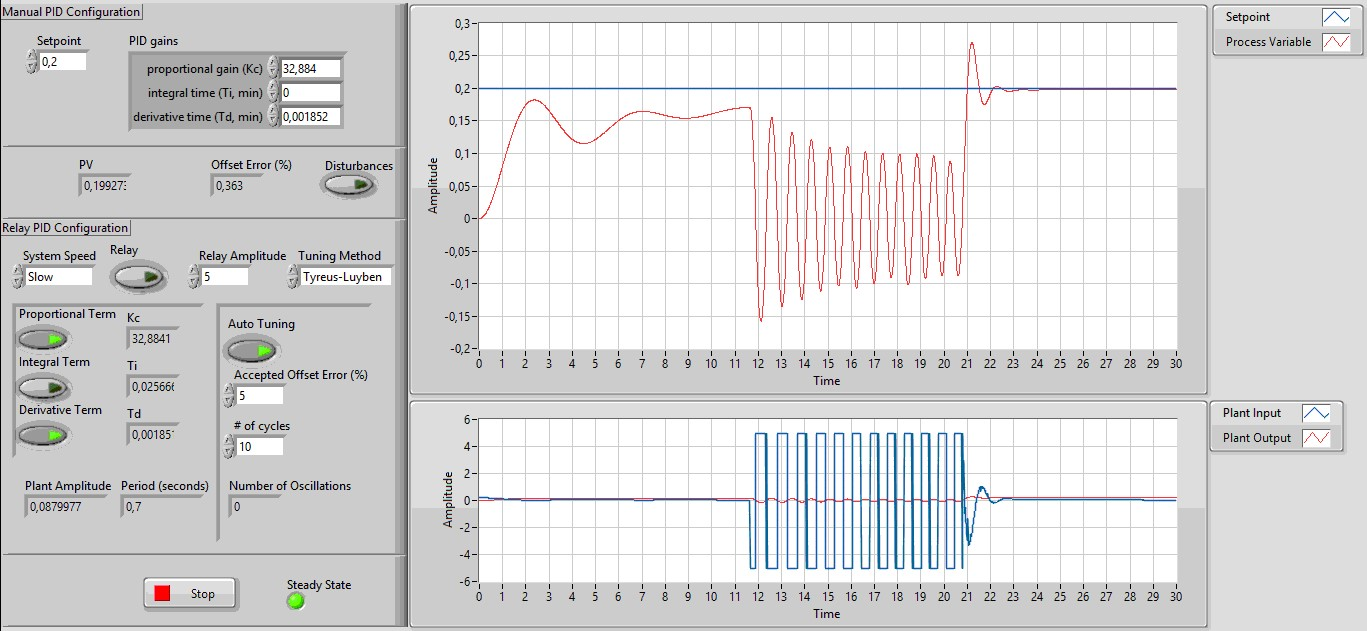
\includegraphics[width=\textwidth,height=5cm,keepaspectratio]{aircraft_pd_TL}
  \caption{Απόκριση του αεροσκάφους σε είσοδο $\delta = 0.2$ rad με τη χρήση αναλογικού -- διαφορικού ελέγχου που τα κέρδη έχουν υπολογιστεί με τους τύπους Tyreus -- Luyben}
  \label{fig:aircraft_pd_TL}
\end{figure}

\subsubsection{Αντιμετώπιση Διαταραχών}

Στο Σχήμα \ref{fig:aircraft_disturbances} φαίνεται η απόκριση του συστήματος υπό την παρουσία στιγμιαίων διαταραχών. Εύκολα γίνεται αντιληπτό ότι ο ελεγκτής παρουσιάζει πολύ καλή συμπεριφορά κάτω από συνθήκες διαταραχών αφού δεν αφήνει την έξοδο του συστήματος να αποκλίνει σχεδόν καθόλου από το επιθυμητό σημείο.

\begin{figure}[h]
  \centering
  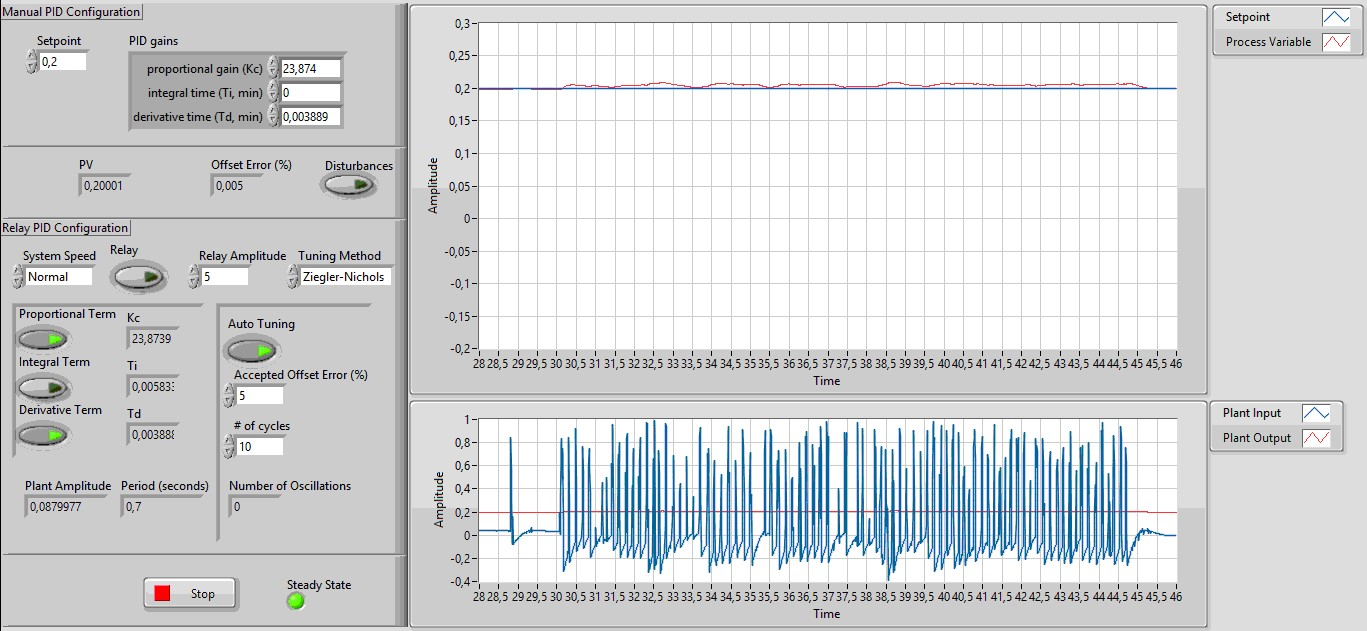
\includegraphics[width=\textwidth,height=5cm,keepaspectratio]{aircraft_disturbances}
  \caption{Απόκριση του συστήματος στην παρουσία διαταραχών με χρήση αναλογικού -- διαφορικού ελέγχου}
  \label{fig:aircraft_disturbances}
\end{figure}

\subsection{Συμπεράσματα}

Σε αυτή την ενότητα το σύστημα που ήταν υπό έλεγχο ήταν αυτό ενός αεροσκάφους. Επειδή οι εξισώσεις που διέπουν τη δυναμική και την κίνηση ενός αεροσκάφους είναι περίπλοκες έγιναν κάποιοι συμβιβασμοί. Έτσι, καταλήξαμε σε μια γραμμική εκτίμηση του συστήματος που μας έδωσε τη συνάρτηση μεταφοράς που φαίνεται στην εξίσωση \ref{eq:aircraft_tf}. Ως στόχοι του ελέγχου τέθηκαν η μικρή υπερακόντιση, ο γρήγορος χρόνος ανύψωσης και το μικρό σφάλμα μόνιμης κατάστασης.

Το πρώτο πράγμα που ελέγχθηκε ήταν η απόκριση του συστήματος χωρίς τη χρήση ελεγκτή. Αυτή γρήγορα κρίθηκε μη ικανοποιητική καθώς δεν πληρούσε κανένα από τα κριτήρια ελέγχου. Στη συνέχεια, χρησιμοποιήθηκε ο αναλογικός όρος του ελεγκτή. Παρόλο που αυτός βελτίωσε αισθητά το σφάλμα μόνιμης κατάστασης, χειροτέρευσε τα μεταβατικά φαινόμενα του συστήματος και οδήγησε σε υψηλό ποσοστό υπερακόντισης και σε εκτεταμένες ταλαντώσεις. Επειδή το σύστημα έχει από μόνο του έναν πόλο στο μηδέν, το σφάλμα μόνιμης κατάστασης θα τείνει να μηδενιστεί χωρίς τη χρήση ολοκληρωτικού όρου. Συνεπώς, προστέθηκε ο διαφορικός όρος στον ελεγκτή για τη βελτίωση της ευστάθειας του αεροσκάφους. Με τη χρήση αναλογικού -- διαφορικού ελέγχου οι ταλαντώσεις εξαφανίστηκαν, η υπερακόντιση έγινε πολύ μικρή και το σφάλμα συγκλίνει πιο γρήγορα στο μηδέν ενώ και οι χρόνοι ανύψωσης και ηρεμίας μειώθηκαν αισθητά. Τέλος, ο έλεγχος παρουσιάζει πολύ καλή συμπεριφορά υπό τη συνθήκη διαταραχών. Συνοψίζοντας, ο αυτο--ρυθμιζόμενος PID ελεγκτής κατάφερε να ελέγξει πολύ ικανοποιητικά το σύστημα του αεροσκάφους.\newpage

\section{Σύστημα Beam \& Ball}

\subsection{Εισαγωγή}

Το τελευταίο σύστημα που θα προσπαθήσουμε να ελέγξουμε είναι το σύστημα Δοκός -- Σφαίρα όπως αυτό φαίνεται στο Σχήμα \ref{fig:bb2}. Μία μπάλα τοποθετείται σε μία δοκό όπου επιτρέπεται να κυλήσει με ένα βαθμό ελευθερίας κατά μήκος της δέσμης. Ένας μοχλοβραχίονας είναι στερεωμένος στη δοκό στο ένα άκρο και ένα σερβο γρανάζι στο άλλο. Καθώς ο σερβομηχανισμός γυρίζει σε γωνία $\theta$, ο μοχλός αλλάζει τη γωνία της δέσμης κατά $\alpha$. Όταν αλλάζει η γωνία από την οριζόντια θέση, η βαρύτητα προκαλεί την κύλιση της σφαίρας κατά μήκος της δέσμης. Ένας ελεγκτής θα σχεδιαστεί για αυτό το σύστημα έτσι ώστε να μπορεί να χειραγωγηθεί η θέση της μπάλας.

\begin{figure}[h]
  \centering
  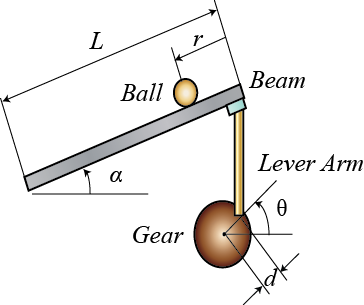
\includegraphics[width=\textwidth,height=5cm,keepaspectratio]{bb2}
  \caption{Μοντέλο συστήματος Δοκός -- Σφαίρα}
  \label{fig:bb2}
\end{figure}

\subsection{Μαθηματικό Μοντέλο}

Η δεύτερη παράγωγος της γωνίας εισόδου $\alpha$ επηρεάζει στην πραγματικότητα το δεύτερο παράγωγο του $r$. Ωστόσο, θα αγνοήσουμε αυτή τη συμβολή. Η Lagrangian εξίσωση κίνησης για την μπάλα δίνεται από την ακόλουθη εξίσωση
\begin{equation}
0 = \left(\frac{J}{R^2}+m\right)\ddot{r}+mg\sin\alpha - mr\dot{\alpha}^2
\end{equation}
Η παραπάνω εξίσωση είναι μη γραμμική. Σε αυτή την ενότητα θα επιχειρήσουμε να ελέγξουμε, πέρα από τη γραμμική προσέγγιση του συστήματος αυτού, και το μη γραμμικό σύστημα. Αρχικά, θα συνεχίσουμε με τη γραμμική προσέγγιση και μετά τον έλεγχο του γραμμικού συστήματος θα ασχοληθούμε και με το μη γραμμικό.

\subsection{Γραμμικό Μοντέλο}

Γραμμικοποίηση αυτής της εξίσωσης γύρω από τη γωνία της ράβδου, $\alpha = 0$, μας δίνει την ακόλουθη γραμμική προσέγγιση του συστήματος:
\begin{equation}
\left(\frac{J}{R^2}+m\right)\ddot{r} = -mg\alpha
\end{equation}
Η εξίσωση που συνδέει τη γωνία της ράβδου με τη γωνία του γραναζιού μπορεί να προσεγγιστεί ως γραμμική από την παρακάτω εξίσωση:
\begin{equation}
\alpha = \frac{d}{L}\theta
\end{equation}
Αντικαθιστώντας αυτό στην προηγούμενη εξίσωση, παίρνουμε:
\begin{equation}
\left(\frac{J}{R^2}+m\right)\ddot{r} = -mg\frac{d}{L}\theta
\end{equation}
Λαμβάνοντας το μετασχηματισμό Laplace της παραπάνω εξίσωσης, βρίσκουμε την ακόλουθη εξίσωση:
\begin{equation}
\left(\frac{J}{R^2}+m\right)R(s)s^2 = -mg\frac{d}{L}\Theta(s)
\end{equation}
Αναδιατάσσοντας την εξίσωση αυτή βρίσκουμε τη συνάρτηση μεταφοράς από τη γωνία του γραναζιού $\Theta(s)$ στη θέση της μπάλας $R(s)$.
\begin{equation}
P(s) = \frac{R(s)}{\Theta(s)} = -\frac{mgd}{L\left(\frac{J}{R^2}+m\right)}\frac{1}{s^2} \left[\frac{m}{rad}\right]
\end{equation} 
Όπως φαίνεται από τη συνάρτηση μεταφοράς, το παραπάνω μοντέλο έχει διπλό πόλο στο μηδέν οπότε παρουσιάζει αρκετή δυσκολία στον έλεγχό του.

\subsubsection{Πείραμα}

Στο συγκεκριμένο παράδειγμα κάνουμε τις παραδοχές ότι η μπάλα εκτελεί κύλιση χωρίς ολίσθηση κατά μήκος της ράβδου και επίσης ότι η τριβή μεταξύ της μπάλας και της δοκού είναι αμελητέα. Οι παράμετροι του συστήματος δίνονται ως εξής:
\begin{flushleft}
\begin{tabular}{lll}
$\mathbf{m}$ & μάζα της μπάλας & $0.11\ kg$ \\  
$\mathbf{R}$ & ακτίνα της μπάλας & $0.015\ m$ \\ 
$\mathbf{d}$ & απόσταση του μοχλοβραχίονα από το κέντρο του γραναζιού & $0.03\ m$ \\ 
$\mathbf{g}$ & επιτάχυνση της βαρύτητας & $9,8\ \frac{m}{s^2}$ \\ 
$\mathbf{L}$ & μήκος της δοκού & $1\ m$ \\ 
$\mathbf{J}$ & ροπή αδράνειας της μπάλας & $ 9.99*10^{-6}\ kgm^2 $ \\ 
\end{tabular}
\end{flushleft}

\paragraph{Απόκριση Χωρίς Έλεγχο}\hfill

Αρχικά βλέπουμε πώς το σύστημα αποκρίνεται όταν σε αυτό δεν εφαρμόζεται έλεγχος και εισάγουμε μια βηματική είσοδο με πλάτος $\text{setpoint}=0.25\ m$. Αυτό σημαίνει ότι θέλουμε η μπάλα να σταθεροποιηθεί $25\ \text{εκατοστά}$ μακριά από την άκρη της δοκού ή αλλιώς στο $1/4$ του μήκους της. Από το Σχήμα \ref{fig:ball_beam_no_control} εύκολα συμπεραίνουμε ότι το σύστημα είναι οριακά ευσταθές και ότι απαιτείται έλεγχος.

\begin{figure}[h]
  \centering
  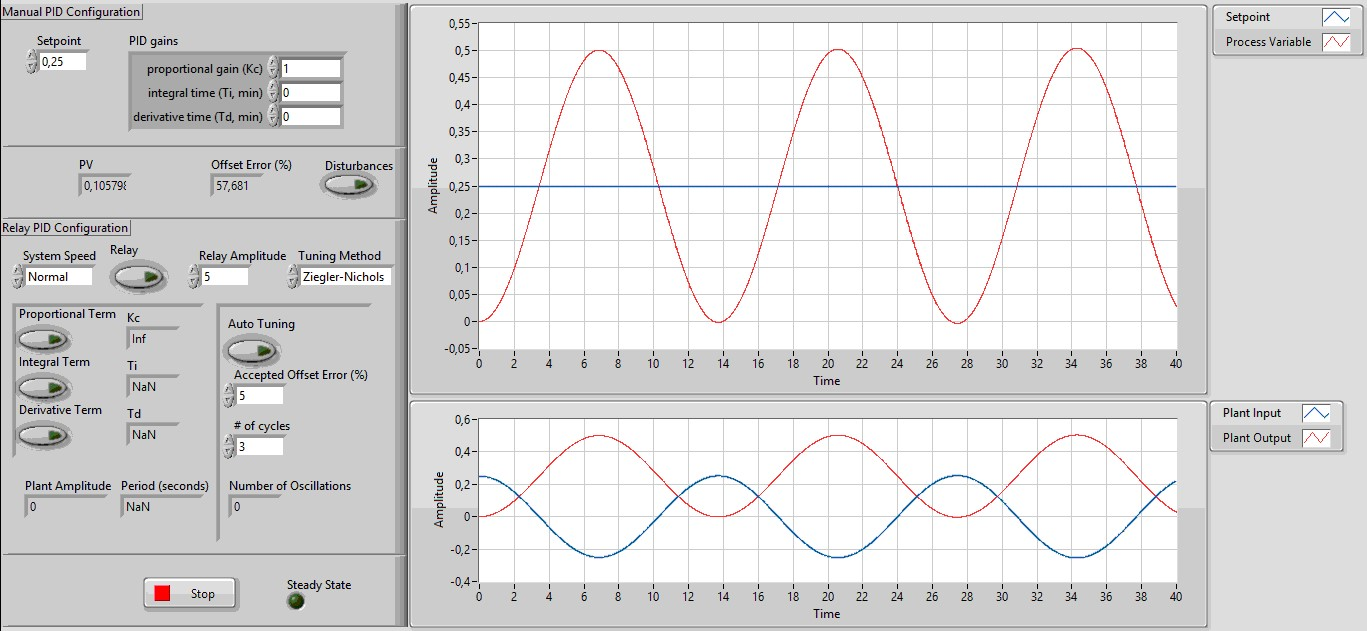
\includegraphics[width=\textwidth,height=5cm,keepaspectratio]{ball_beam_no_control}
  \caption{Βηματική απόκριση του συστήματος δοκού -- σφαίρας χωρίς έλεγχο}
  \label{fig:ball_beam_no_control}
\end{figure}

\paragraph{Αναλογικός Έλεγχος}\hfill

\begin{figure}[h]
  \centering
  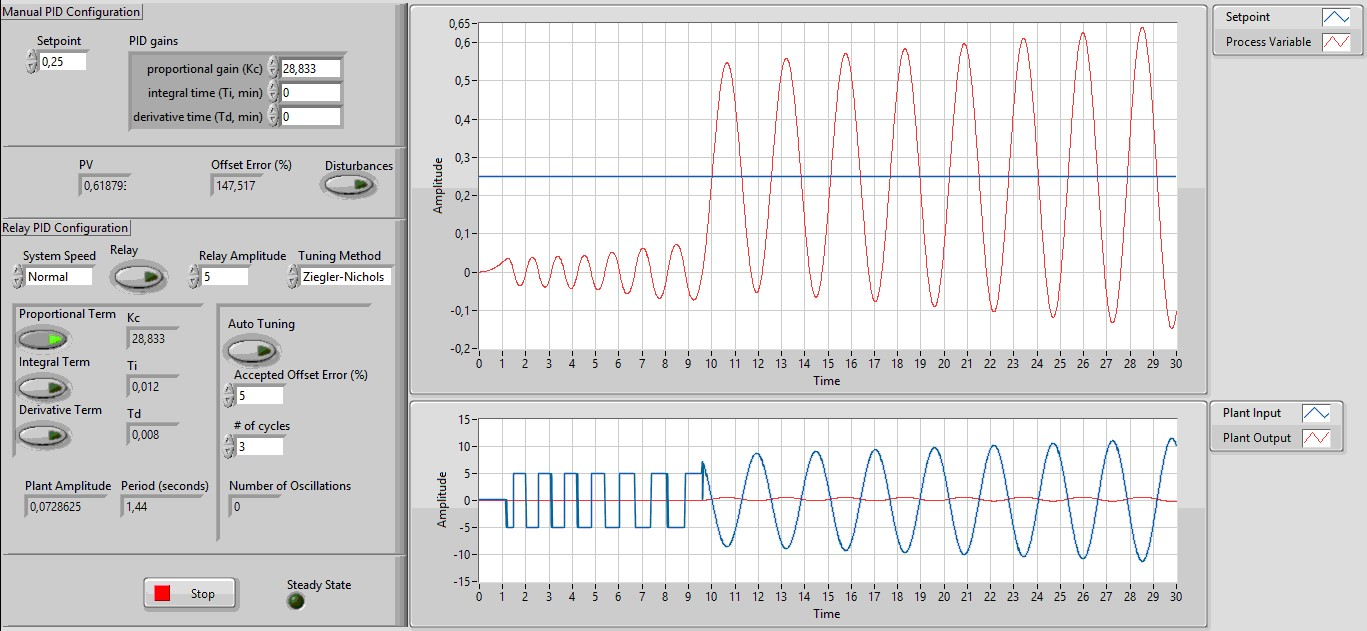
\includegraphics[width=\textwidth,height=5cm,keepaspectratio]{ball_beam_proportional}
  \caption{Βηματική απόκριση του συστήματος δοκού -- μπάλας με χρήση αναλογικού ελέγχου}
  \label{fig:ball_beam_proportional}
\end{figure}

Το Σχήμα \ref{fig:ball_beam_proportional} δείχνει την απόκριση του συστήματος με τη χρήση του αναλογικού όρου του οποίου το κέρδος έχει υπολογιστεί αυτόματα. Βλέπουμε ότι ο αναλογικός όρος όχι απλά δε βελτίωσε την απόκριση αλλά οδηγεί το σύστημα να εκτελεί ταλαντώσεις ολοένα και αυξανόμενου πλάτους. Επίσης, κατά τη διάρκεια του πειράματος relay το σύστημα δεν εισέρχεται σε κύκλο αμείωτων ταλαντώσεων. Αντιθέτως, οι ταλαντώσεις του έχουν πλάτος που αυξάνεται με την πάροδο του χρόνου. Έχει ενδιαφέρον να δούμε την απόδοση του αυτο--ρυθμιζόμενου PID ελεγκτή υπό αυτές τις συνθήκες για ένα απαιτητικό σύστημα σαν αυτό.



\paragraph{Αναλογικός -- Διαφορικός Έλεγχος}\hfill

Για τη βελτίωση της συμπεριφοράς του συστήματος εισάγουμε και το διαφορικό όρο στον ελεγκτή. Όπως φαίνεται στο Σχήμα \ref{fig:ball_beam_pd} το σύστημα με την προσθήκη αυτή έγινε πλέον ευσταθές. Επίσης παρουσιάζει μικρό ποσοστό υπερακόντισης και τείνει γρήγορα στο μηδέν.

\begin{figure}[h]
  \centering
  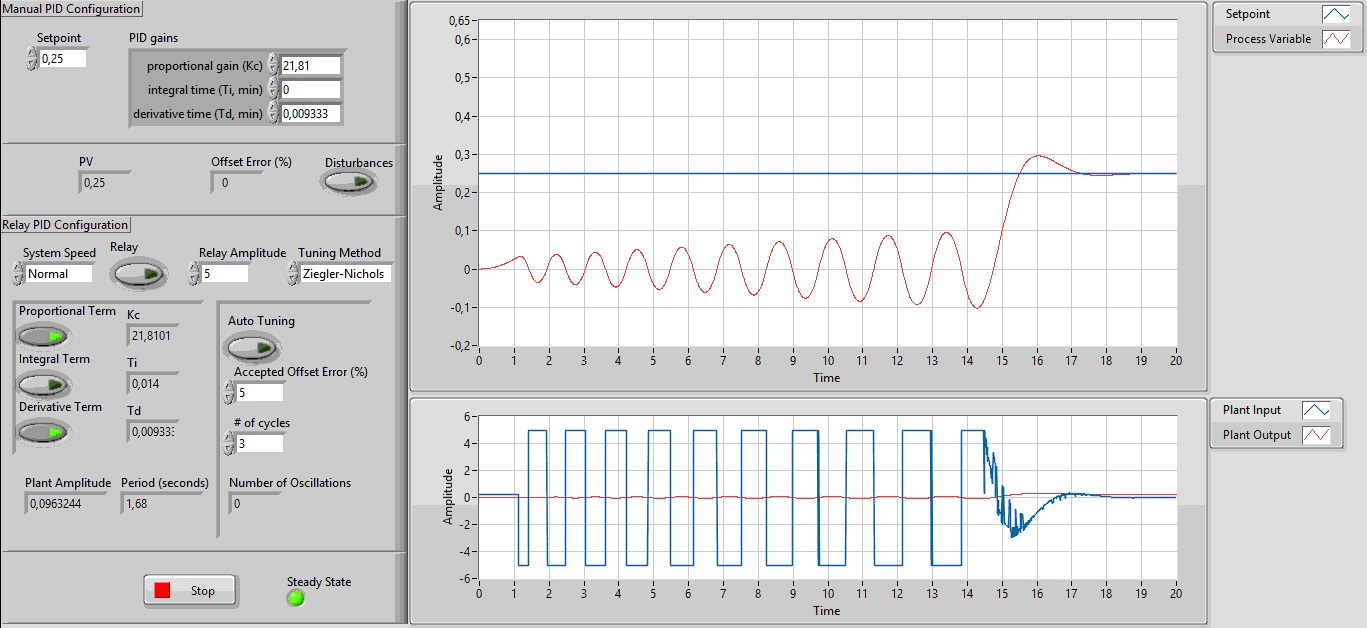
\includegraphics[width=\textwidth,height=5cm,keepaspectratio]{ball_beam_pd}
  \caption{Βηματική απόκριση του συστήματος δοκού -- μπάλας με χρήση αναλογικού -- διαφορικού ελέγχου}
  \label{fig:ball_beam_pd}
\end{figure}

\begin{figure}[h]
  \centering
  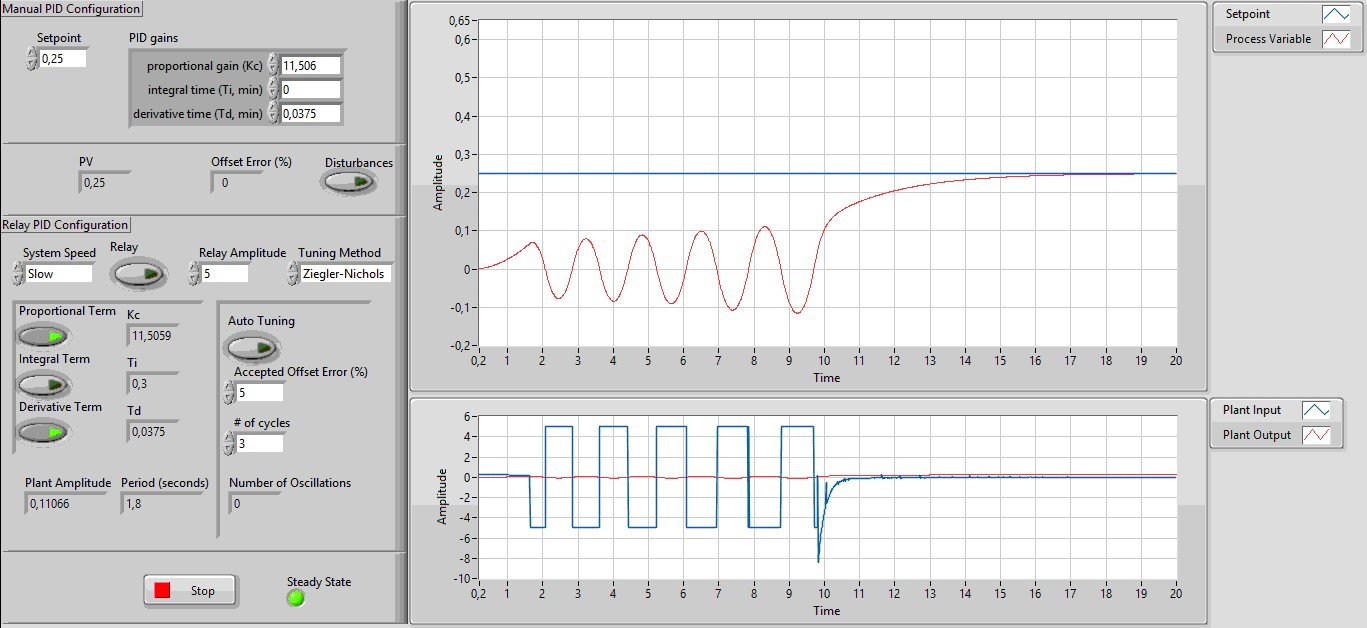
\includegraphics[width=\textwidth,height=5cm,keepaspectratio]{ball_beam_pd_slow}
  \caption{Βηματική απόκριση του συστήματος δοκού -- μπάλας με χρήση αναλογικού -- διαφορικού ελέγχου και επιθυμητή ταχύτητα απόκρισης ``Slow"}
  \label{fig:ball_beam_pd_slow}
\end{figure}

Επίσης στο Σχήμα \ref{fig:ball_beam_pd_slow} φαίνεται πώς το σύστημα αποκρίνεται στην ίδια είσοδο αν η ταχύτητά του έχει οριστεί σε ``Slow". Οι χρόνοι ανύψωσης και ηρεμίας έχουν αυξηθεί αισθητά αλλά το σύστημα πλέον παρουσιάζει μηδενική υπερακόντιση.

\paragraph{Αντιμετώπιση Διαταραχών}\hfill

\begin{figure}[h]
  \centering
  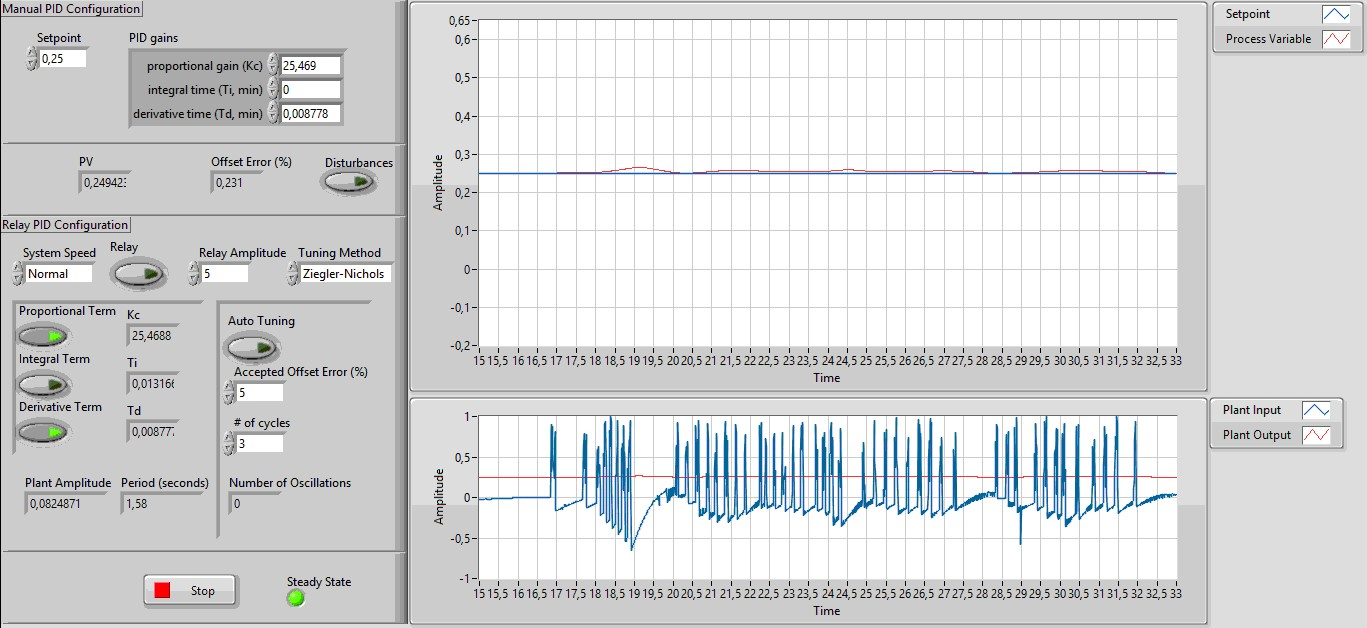
\includegraphics[width=\textwidth,height=5cm,keepaspectratio]{ball_beam_disturbances}
  \caption{Απόκριση του συστήματος στην παρουσία διαταραχών με χρήση αναλογικού -- διαφορικού ελέγχου}
  \label{fig:ball_beam_disturbances}
\end{figure}

Στο Σχήμα \ref{fig:ball_beam_disturbances} βλέπουμε πώς συμπεριφέρεται το σύστημα δοκός -- μπάλα υπό την παρουσία διαταραχών. Εύκολα γίνεται αντιληπτό ότι ο ελεγκτής παρουσιάζει πολύ καλή συμπεριφορά, αφού δεν αφήνει τη μπάλα να κυλίσει μακριά από το επιθυμητό σημείο και επίσης την επιστρέφει σχεδόν αμέσως στη θέση ισορροπίας της.
















